\documentclass[12pt,titlepage]{article}
\usepackage[a4paper,top=3cm, bottom=3cm, left=2.5cm, right=2.5cm]{geometry}
\usepackage{parskip}
\setlength{\parindent}{0cm}
\usepackage{microtype} % improves typography or something idk
\usepackage[utf8]{inputenc}
\usepackage[T1]{fontenc}
\usepackage[australian,british]{babel}
\usepackage{soul} % strikeout text
\usepackage{times}
\usepackage{subfiles}
\usepackage{emptypage}
\usepackage{xspace} % for spaces after custom commands
\usepackage{tocloft}
\usepackage{mathtools}
\usepackage[table]{xcolor}
\usepackage{lipsum}
\usepackage{graphicx}
\usepackage{float}
\usepackage{tikz}
\usepackage{amsmath}
\usepackage{subcaption}
\usepackage{longtable}
\usepackage{algorithm}
\usepackage[noend]{algpseudocode}

\begin{document}

\begin{titlepage}
    \newgeometry{margin=3cm}
	\centering
    
\includegraphics[width=0.5\linewidth]{Images/epfl.png}\\[0.25cm] 	% University Logo
    \textsc{\LARGE École Polytechnique Fédérale de Lausanne}\\ \vspace{5cm}
    \textsc{\LARGE Semester Project Report}\\ \vspace{2cm}
    \textsc{\Large Control and Identification of Hovercraft}\\ 
    \vspace{4cm}
    \textsc{\large \textit{Submitted by}}\\ 
    \vspace{7pt}
    \textsc{\large Anirvan Dutta}\\
    \vspace{1cm }
    \textsc{\large  \textit{Supervisor}}\\ 
    \vspace{7pt}
    \textsc{\large Yingzhao Lian}\\
    \vspace{1cm}
    \textsc{\large  \textit{Submitted to}}\\ 
    \vspace{7pt}
    \textsc{\large Prof Colin Jones}\\
    \vspace{1cm}
    
    
    \vspace{\fill}
    \today
\end{titlepage}
\restoregeometry

\tableofcontents
\newpage

\section{Acknowledgement}
I would like to express my sincere gratitude towards several people who guided and helped in the completion of this semester project. 

First and foremost, I would like to thank Yingshao Lian for his guidance and support in building the prototype and development of the identification framework. I would also like to thank Christophe Salzmann and Peter Listov for helping me with the booking and setup of the tracking room. Additionally, I would like to thank my dear colleague Sujal Amrit Topno who helped me build the CAD model of the developed prototype. 

Finally, I would like to thank Prof. Colin Jones for his supervision and support throughout the project.

\newpage

\section{Introduction}
A hovercraft is an under-actuated system with 3 degrees of freedom and 2 active degree of control. It is supported by a cushion of air and moves by propeller thrust, involving nonlinear dynamics. 
In order to control a hovercraft, it is crucial of know the parameters involved in the dynamic model. The objective of this project is to overcome the previous challenges in design and identification of a miniaturized hovercraft model and propose a working solution. 
\subsection{Previous Work}
Prior development comprised of a miniaturized hovercraft based on `TinyWhoover' design as shown in Fig.\ref{fig:prev_hard_1} \cite{b2} and micro quadcopter based design as shown in Fig.\ref{fig:prev_hard_2}. The `TinyWhoover' prototype had a major drawback of providing thrust only in forward direction, limiting the controllability of the hovercraft. Additionally, the motors suffered from vibration of the foam mounts, making the hardware demonstrate complex dynamics. The second prototype included a backward set of motors to provide thrust in opposite direction, however it relied on external air cushion provided by a hockey table, making deployment and scaling an issue. In order to overcome the above mentioned challenges, a novel miniaturized hovercraft was developed. 

\begin{figure}[H]
    \centering
\begin{minipage}{.5\textwidth}
  \centering
    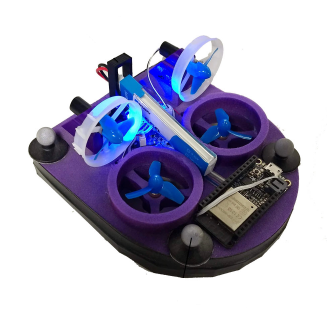
\includegraphics[width=0.95\columnwidth]{Images/previous_hov_1.PNG}\\
    \caption{TinyWhoover hovercraft design \cite{b2}}
    \label{fig:prev_hard_1}
    \end{minipage}%
\begin{minipage}{.5\textwidth}
  \centering
    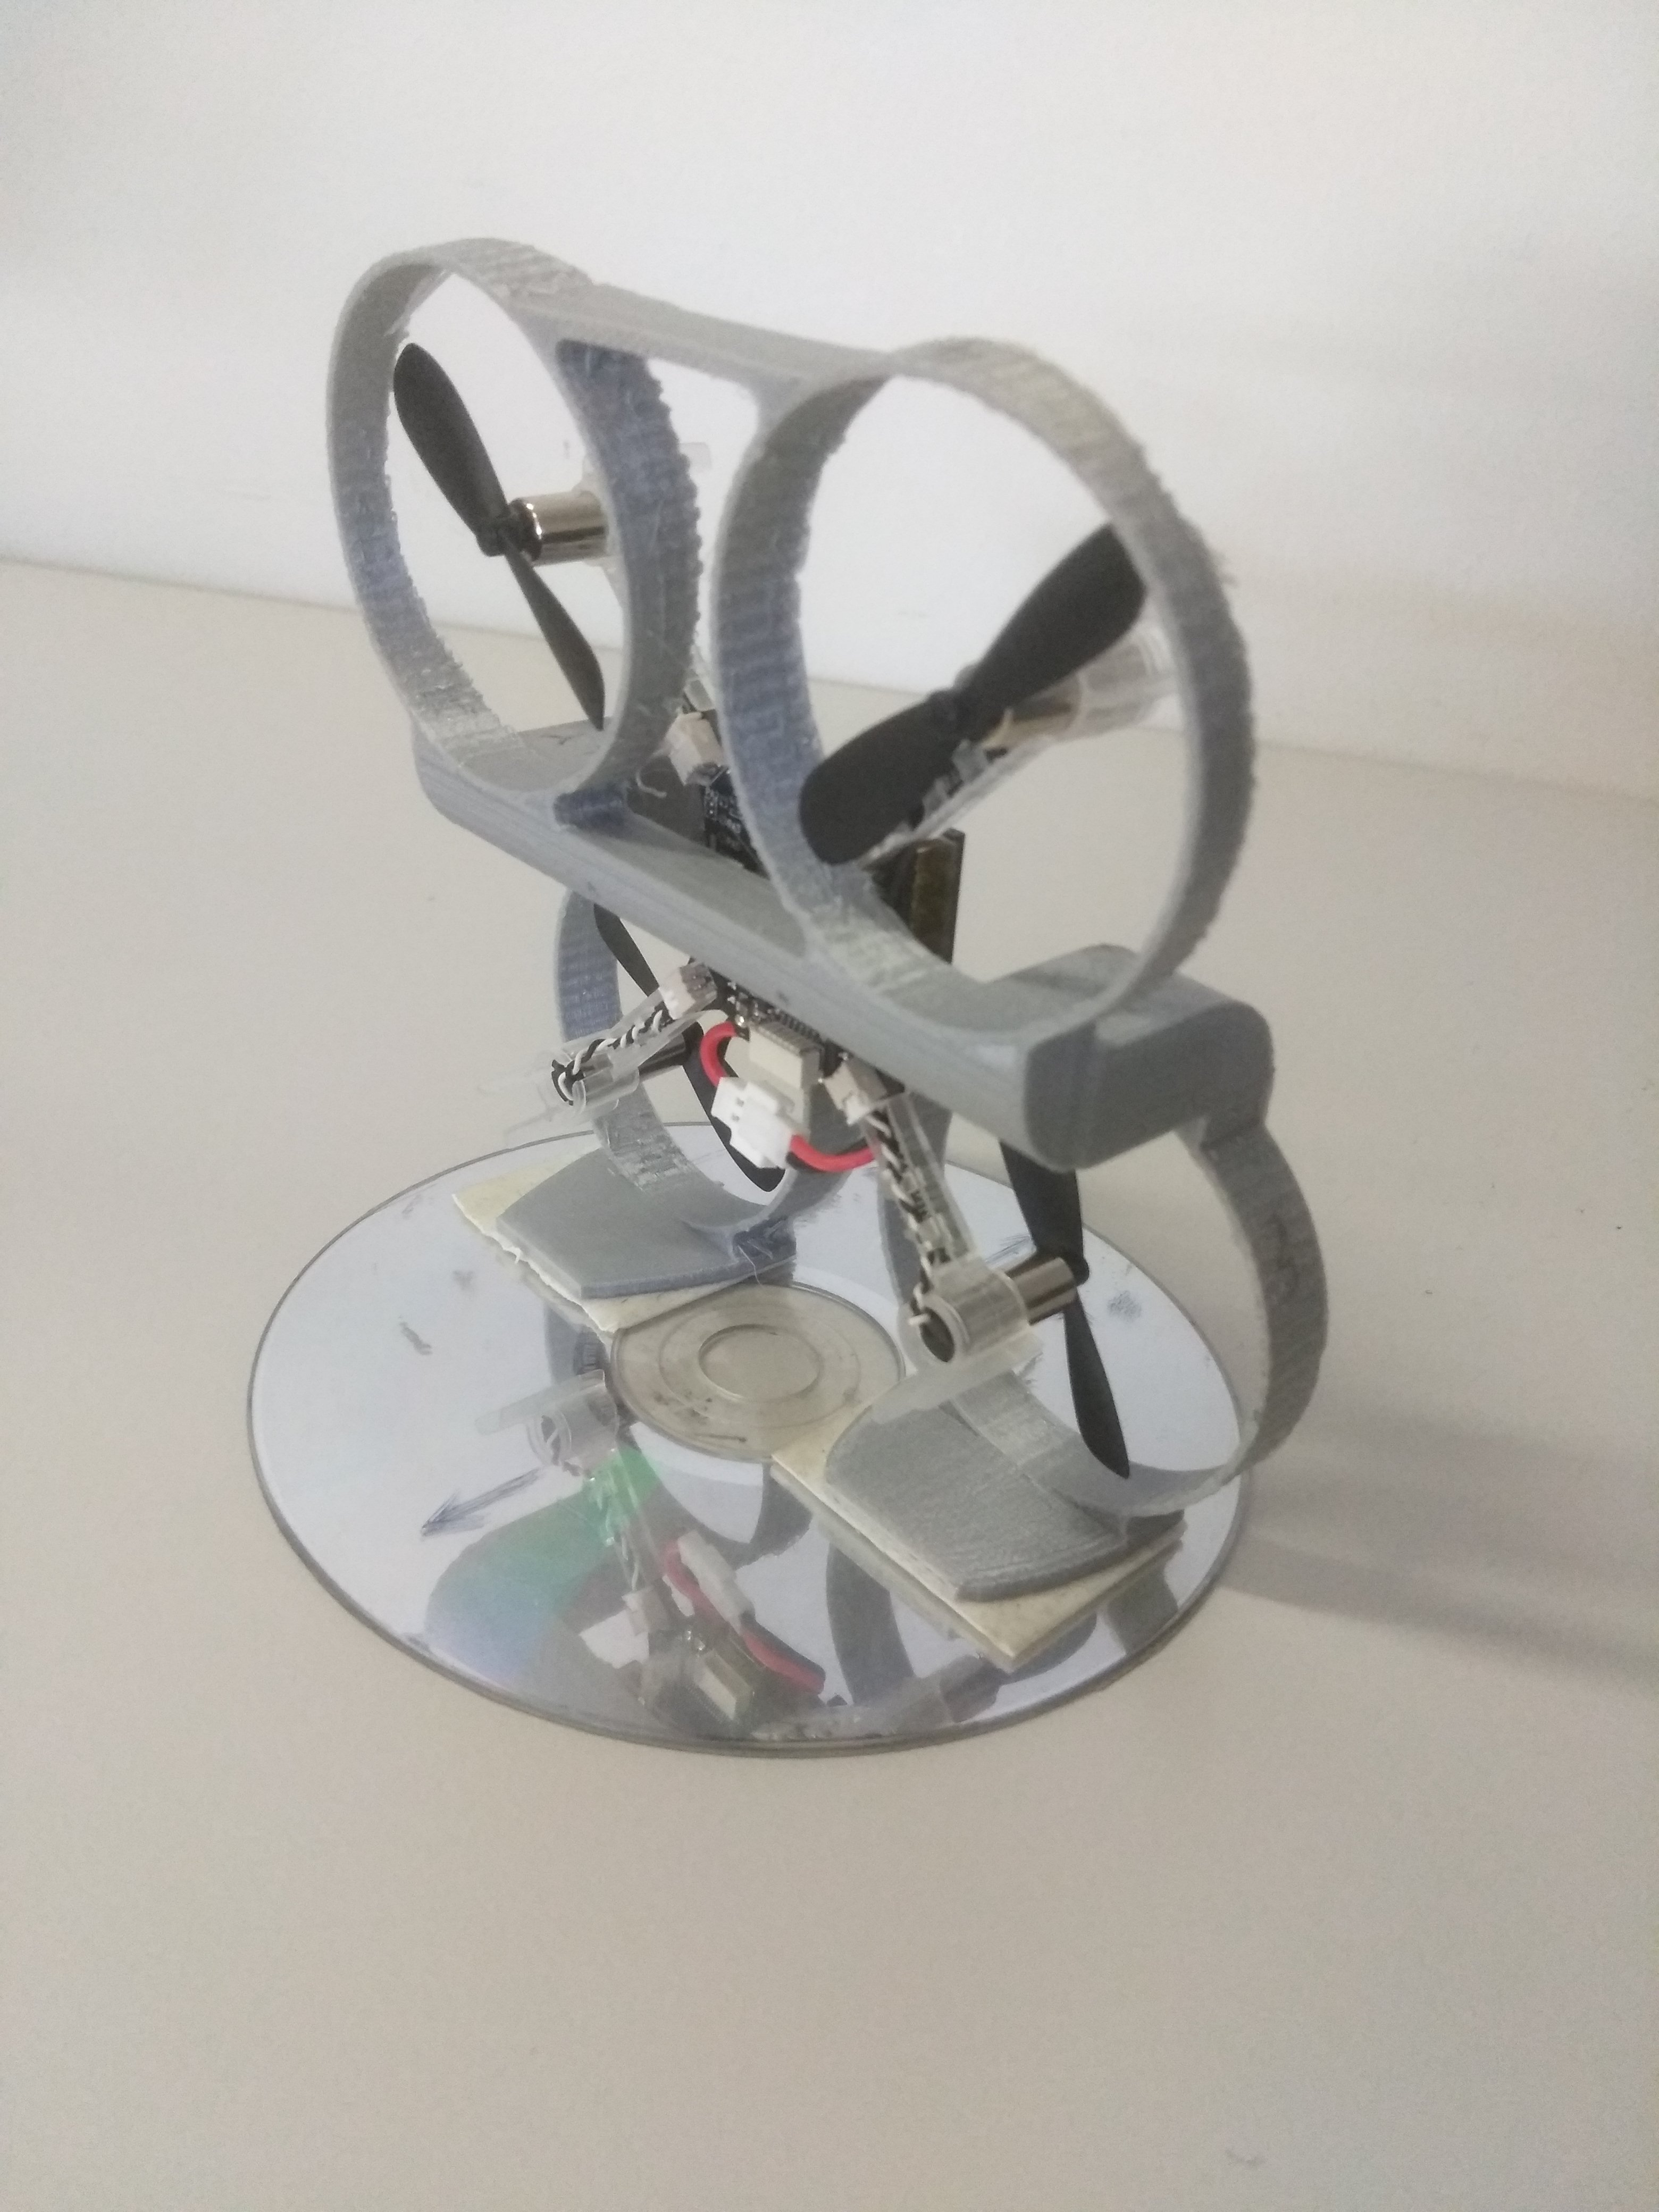
\includegraphics[width=0.74\columnwidth]{Images/airhockey.jpg}\\
    \caption{Air hockey hovercraft design}
    \label{fig:prev_hard_2}
    \end{minipage}%
\end{figure}

\section{Hardware Design}
In the following section thorough hardware development, modelling and identification framework implemented is presented. The requirements for the hardware were to include forward and backward set of propellers to accelerate and de-accelerate. Along with this, an additional set of propellers were required to control the rotation of the hovercraft. Finally, two sets of lift propellers were required to create a air cushion beneath the hovercraft and also ensure that the moment created by the lift propellers cancel each other out. The proposed design was motivated from a skid steer differential drive mobile base. It not only satisfies the above requirements, but also decouples the 2 active degree of control. Additionally, placement of the propellers were symmetric, ensuring the rotation of the hovercraft about its center of mass and thus, following the theoretical dynamics closely. 

\subsection{CAD model}
The CAD model developed in SolidWorks based on the design requirements. The 3D mesh view of the proposed design is presented in Fig.\ref{fig:cad}.

\begin{figure}[H]
    \centering
    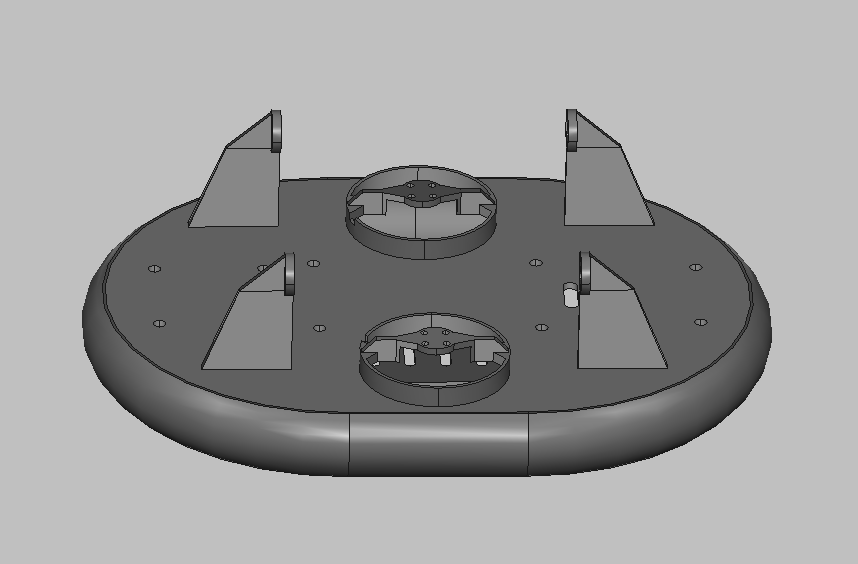
\includegraphics[width=0.8\columnwidth]{Images/proposed_hardware_model.PNG}\\
    \caption{Proposed hardware model of the hovercraft}
    \label{fig:cad}
\end{figure}

\subsection{Components}
Component selection was crucial and quite challenging for the development of the prototype. Due to additional motors and propellers, it was essential to ensure, the thrust capability of the lift propellers was sufficient to create a air cushion. Secondly, previous hardware utilised off the self beta-flight controller to control motors, however, due to lack of availability of 6 motor controller, a custom solution using 2 set of 4 in 1 electronic speed controller used for micro quadcopters was utilised. Additionally, it was important to select components which were lightweight, have a small footprint and are compatible with each other. The final components used in the development of the prototype are presented in Table.\ref{component}.
\newpage

\begin{center}
\begin{longtable}[c]{|c|c|c|c|}
\hline \rowcolor{gray!30}
S.No. & Part Functionality & Part Name & Quantity \\ \hline
\endfirsthead
\endhead
1 & Motors & \textsc{BETAFPV} 1103 11000kv Brushless Motors   &6  \\ \hline
2 & Motor Drivers & \textsc{Hobbywing} XRotor 12A 4IN1 1-4S Micro ESC & 2 \\ \hline
3 & Propellers & \textsc{BETAFPV} 40mm 4-Blade Props & 6 \\ \hline
4 & Batteries & Lipo Battery Gaoneng GNB HV 650mAh 60C - 2s & 1 \\ \hline
5 & Embedded Board & Adafruit HUZZA32 Feather & 1 \\ \hline 
\caption{Electronic component used in the hovercraft}
\label{component}
\end{longtable}
\end{center}

\subsection{Firmware}
As previously mentioned, a custom firmware was required to be developed in order to control the brushless motors. The embedded board utilised in the hardware was ESP32. The brushless motors were controlled by electronic speed controllers (ESC's) which required pulse width modulated (PWM) signals and cannot be controlled directly by the embedded board. The crux of the firmware relied on the ability to generate appropriate PWM signals using the embedded board to give neccessary speed commands to the ESC's. In order to implement PWM generation, a modified version of the servo library in Arduino IDE was utilised to program the embedded board. The library provided function \texttt{writeMicroseconds(val)}, which provides pulses of 0.02 sec duration with high duration specified in \textit{val} in microseconds. The ESC's were calibrated to take in pulses of range 1000-2000 $\mu sec$, with 1000 being no rotation and 2000 signifying maximum achievable RPM of the brushless motor. The motor thrust identification was also performed to map pulse duration to thrust and is discussed in the \textit{Experiments} section. Throughout the report, \texttt{val} will be denoted as the PWM signal for each motor which serves as the input.

Additionally, in order to control the hovercraft over wireless network, a ROS serial node in Arduino environment was also established in the embedded board. This ensured ease of connecting to the hovercraft and sending motor commands over wireless network from a remote PC. The firmware developed had the following functionalities - 
\begin{itemize}
    \item Calibration of the ESC's to ensure complete range of the brushless motor rotational speed is achieved.
    \item Connection to ROS master server via wireless network whenever master node is active. 
    \item Receive propeller thrust commands from remote computer running ROS master server and translate it to pwm signals
    \item Broadcast current hovercraft status comprising of current motor speeds and time stamp. 
\end{itemize}

\subsection{Developed Prototype}
The final prototype of the proposed hardware was developed and worked as expected and fulfilled the requirements of miniature hovercraft model. The skirt of the CAD model was modified for ease of printing using 3D printer. It weighed a total of 0.176 Kg including the battery. 
\begin{figure}[H]
    \centering
\begin{minipage}{.5\textwidth}
  \centering
    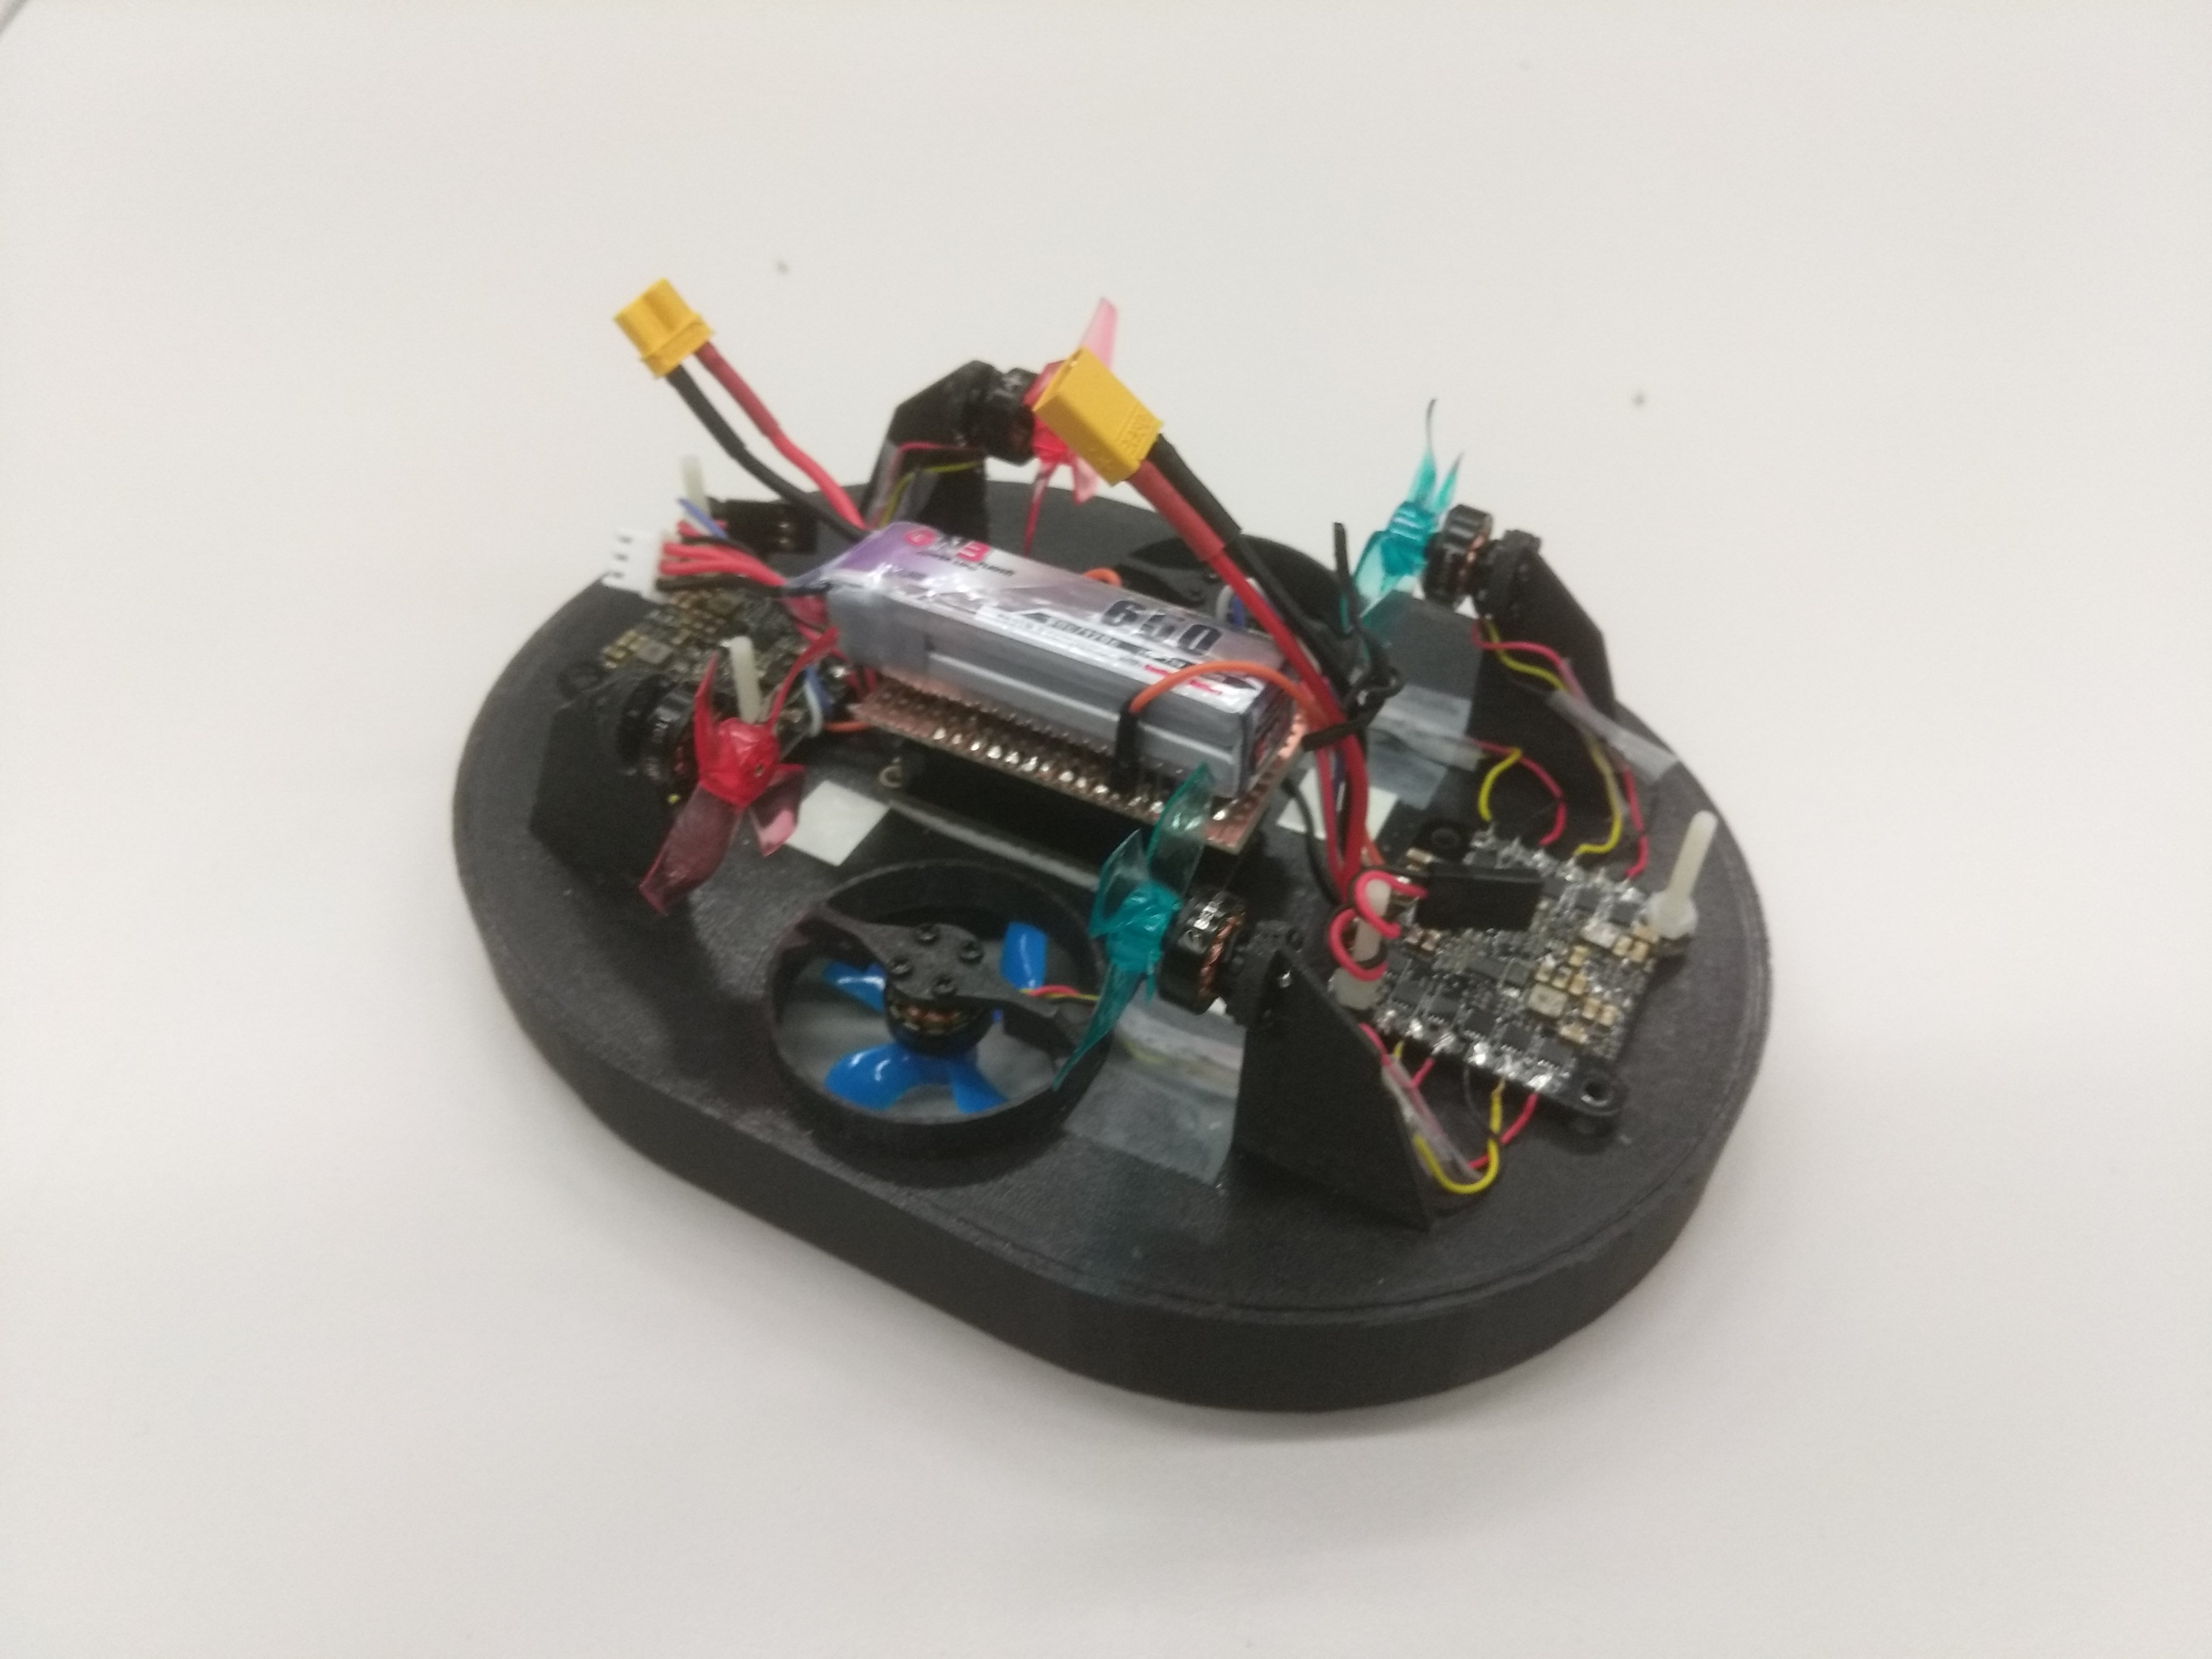
\includegraphics[width=0.9\columnwidth]{Images/sideview_hov.jpg}\\
    \caption{Side View of finished protoype}
    \label{fig:proto_1}
    \end{minipage}%
\begin{minipage}{.5\textwidth}
  \centering
    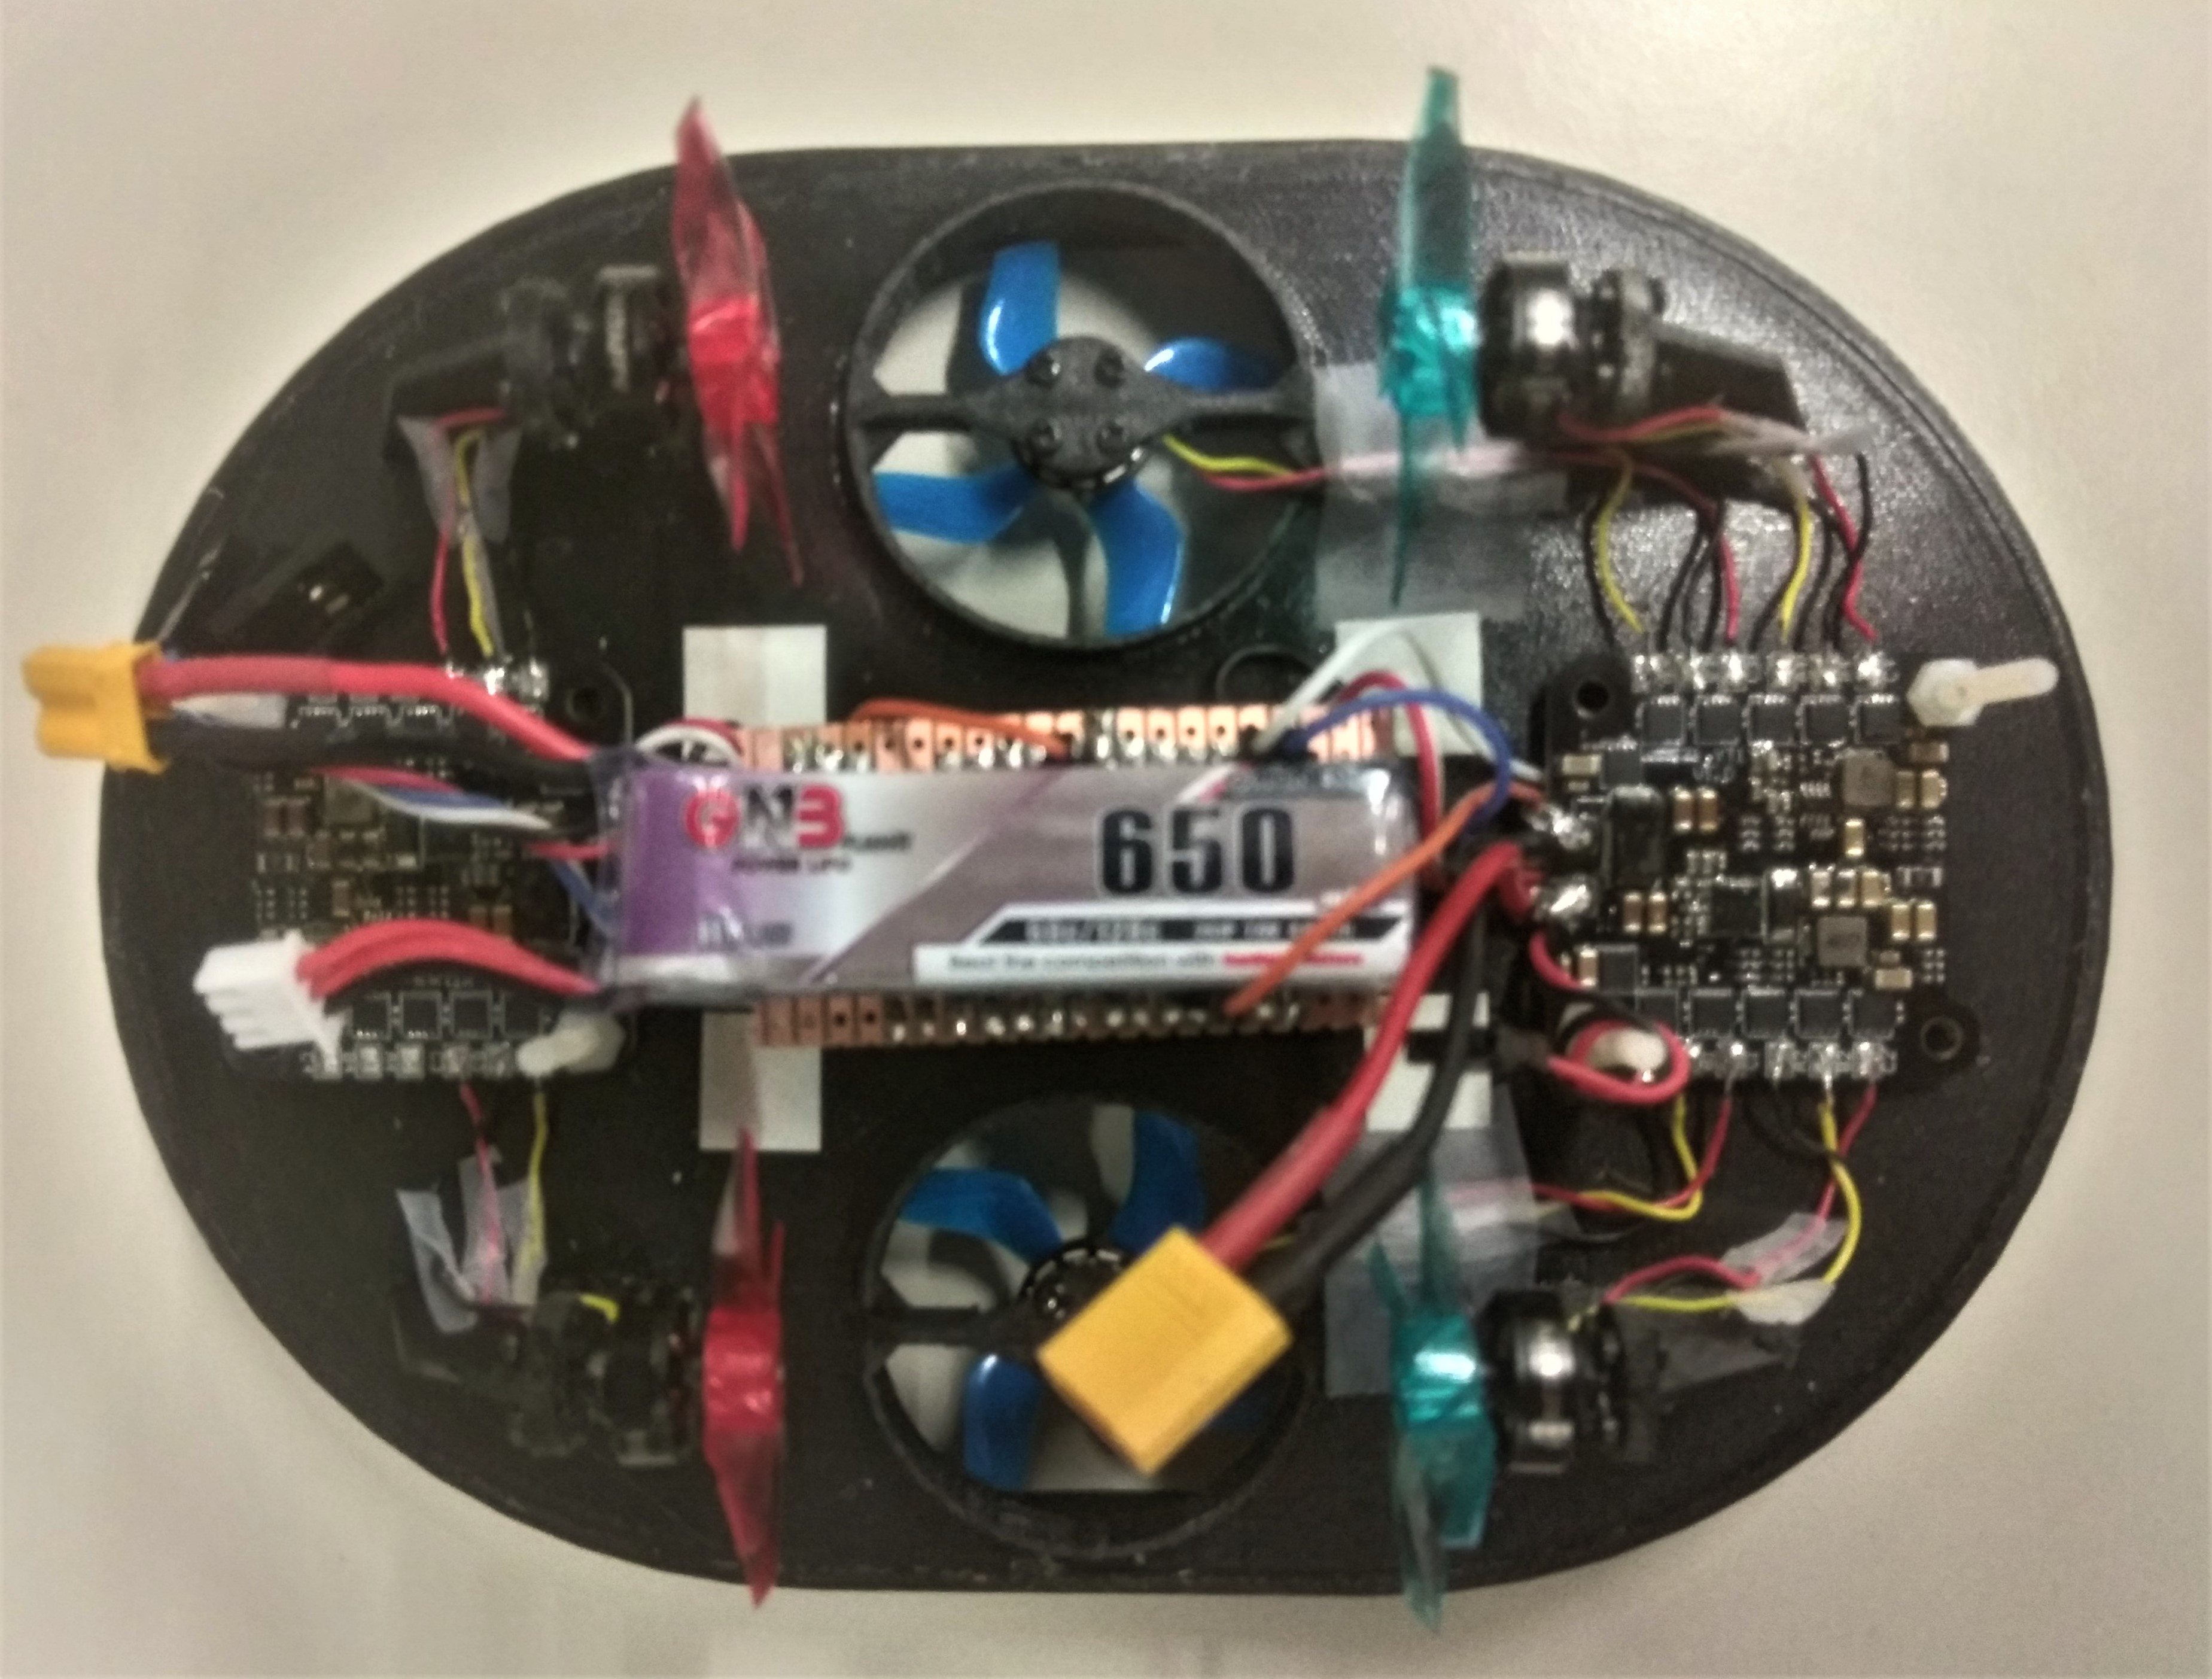
\includegraphics[width=0.9\columnwidth]{Images/topview_hov.jpg}\\
    \caption{Top View of finished protoype}
    \label{fig:proto_2}
    \end{minipage}%
\end{figure}

\section{Modelling and Simulation}
\subsection{System Modelling }
The hovercraft's dynamic model is based on the surface ship model \cite{b1} which follows the standard notation conventions for maritime vehicles. It allows expressing the hovercraft's position as well as its linear and angular velocities with the provided propeller thrust as inputs. The existing model was augmented to include thrust from the four propellers in proposed design. In order to model the hovercraft, two co-ordinate frames are utilised. One attached to the inertial frame of reference denoted as the world-fixed frame $[X_o,Y_o,Z_o]$ and other attached rigidly to the center of mass of the hovercraft denoted as the body fixed frame $[X_b,Y_b,Z_b]$. The z-axes are selected to point inside the plane and the $X_b$ is aligned with the hovercraft's forward direction. The position of hovercraft is expressed in the world frame, while the linear and angular velocity is expressed in the body frame. The notation of the frames are vizualised in Fig.\ref{fig:sysmodel}. The complete state of the hovercraft can be expressed in a vector of 6 dimension. 

\begin{align}
X = 
\begin{bmatrix}
    \eta \\
    \nu \\
\end{bmatrix}
=
\begin{bmatrix}
    x \\
    y \\
    \psi \\
    u \\
    v \\
    r \\
\end{bmatrix}
\end{align}

Where, $\eta=[x,y,\psi]^T$ denotes the position and $\nu=[u,v,r]^T$ denotes the velocity. The inputs of the model in this designed can be represented as - 

\begin{align}
\gamma = 
\begin{bmatrix}
    t_{bl} \\
    t_{br} \\
    t_{fl} \\
    t_{fr} \\
\end{bmatrix}
\end{align}

where subscript $b$ is denoted for \textit{backward}, $l$ for \textit{left}, $r$ for \textit{right} and $f$ for \textit{forward}. The lift thrust are not modelled as it does not play role in planar dynamics and are assumed to be constant. 

\begin{figure}[H]
    \centering
    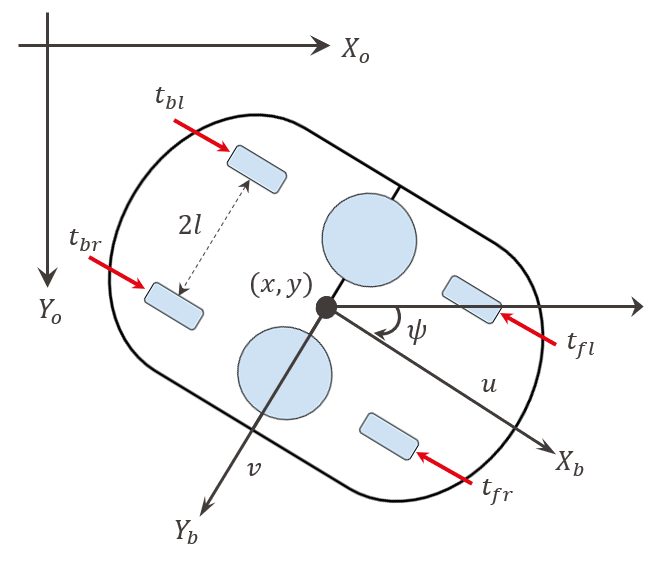
\includegraphics[width=0.5\columnwidth]{Images/hovercraft_model.PNG}\\
    \caption{System model of the hovercraft}
    \label{fig:sysmodel}
\end{figure}

The position and velocity expressed in the Eq.(1) is related by the rotation matrix defined about the z-axis. 

\begin{align}
\dot{\eta} = f_\eta(\nu) = R_z(\psi)\nu =
\begin{bmatrix}
    cos(\psi) & -sin(\psi) & 0 \\
    sin(\psi) & cos(\psi) & 0 \\
    0 & 0 & 1 \\
\end{bmatrix}
\begin{bmatrix}
    u \\
    v \\
    r \\
\end{bmatrix}
\end{align}


The equations of the motion of the hovercraft can be formulated using the Euler Lagrange formulation and can be expressed as - 

\begin{subequations}
\begin{alignat}{2}
    & M\dot{\nu} + C(\dot{\nu})\nu + D\nu = B\gamma \\
    & \dot{\nu} = f_\nu(\nu,\gamma) = M^{-1}(B\gamma - C(\dot{\nu})\nu - D\nu)
\end{alignat}
\end{subequations}
    

Where $M$ is the symmetric inertia matrix, $C$ is the Coriolis matrix, $D$ is the symmetric damping matrix, $B$ is the control matrix and $\gamma$ is the control vector. The $M$ matrix is expressed as - 

\begin{align}
M = 
\begin{bmatrix}
    m & I_{xy} & I_{xz} \\
    I_{yx} & m & I_{yz} \\
    I_{zx} & I_{zy} & I_{z} \\
\end{bmatrix}
= 
\begin{bmatrix}
    m & 0 & 0 \\
    0 & m & 0 \\
    0 & 0 & I_{z} \\
\end{bmatrix}
\end{align}
\newpage 

The $C$ matrix is defined as - 

\begin{align}
C = 
\begin{bmatrix}
    0 & 0 & -mv \\
    0 & 0 & mu \\
    mv & -mu & 0 \\
\end{bmatrix}
\end{align}

The $D$ matrix includes the damping forces along the body co-ordinate frame $[X_b,Y_b,Z_b]$ as $[X_u, Y_v, N_r]$

\begin{align}
D = 
\begin{bmatrix}
    X_u & 0 & 0 \\
    0 & Y_v & 0 \\
    0 & 0 & N_r \\
\end{bmatrix}
\end{align}
The B matrix transforms the thrust from the four propellers into acceleration in body co-ordinate frame. 

\begin{align}
B =
\begin{bmatrix}
    1 & 1 & -1 & -1\\
    0 & 0 & 0 & 0\\
    l & -l & -l & l \\
\end{bmatrix}
\end{align}

Clearly, the hovercraft model still remains under-actuated, however we now have independent control over translation and rotation as the rank of matrix $B$ is 2, due to additional set of motors in front of the hovercraft, giving backward thrust. 

\subsection{Simulation}
In order to implement control or identification from a computer, it is essential to discretize the continuous dynamic equation formulated in the previous section. Based on the previous work, fourth-order Runge Kutta (RK4) method is used for numerical intergration, with $h=0.01$.

\begin{subequations}
\begin{alignat}{2}
& \eta_{sim}(t_{k+1}) = RK4(f_\eta,\nu_{sim}(t_k)) \\
& \nu_{sim}(t_{k+1}) = RK4(f_\nu,\nu_{sim}(t_k),\gamma_k) \\
& t_{k+1} - t_k = h
\end{alignat}
\label{eq:RK4}
\end{subequations}


\section{Identification Framework}
Based on the formulation of the model, the parameters of the hovercraft model can be expressed in the following vector. 
\begin{align}
    \theta = [m,l,I_z,X_u,Y_v,N_r]
\end{align}
In this, $m$ and $l$ can be measured quite accurately, however, $I_z,X_u,Y_v,N_r$, are difficult to measure or account for. This raises the need for development of identification framework. In this project, two popular framework has be utilised to identify the unknown parameters. These are described subsequently. 

\subsection{Offline Identification}
In this framework, the idea is to minimize the absolute value of the difference between simulated velocity trajectory and actual velocity for a known input to the hovercraft thrusts. This framework is offline, as complete trajectory is stored and is later used to optimise the unknown parameters. The framework can be formulated as - 

\begin{equation}
\theta^* = \underset{\theta}{\operatorname{argmin}} \frac{1}{N}\sum_{k=1}^{N}|w.\nu_{sim}(t_k,\theta) - \nu_{meas}(t_k)|
\end{equation}
where, $w$ is a weighing factor to account for different scales of $\nu$. 
\begin{equation}
    w = 
    \begin{bmatrix}
        \frac{1}{\sigma_u} & \frac{1}{\sigma_v} & \frac{1}{\sigma_r} \\
    \end{bmatrix}^T
\end{equation}
where, $\sigma_u, \sigma_v, \sigma_r$ are the empirical standard deviation of the measured terms in $\nu_{meas}$
As the optimization problem stated above is nonconvex, \texttt{fmincon} function of \textsc{matlab} was used to implement this formulation. Along with the optimization problem implementation, one also had to consider the fact that the simulated velocity trajectory was generated using RK4 integration using step time of $h=0.01$, however, the actual data being sampled had a much lower sampling time, therefore following the previous work, upsampling of measured velocity was also implemented using standard interpolation technique. 

The algorithm for offline parameter identification was based on the previous work in \cite{b2}. 


\subsection{Online Identification}
In online parameter identification, both states and parameters are estimated simultaneously. In general, the online identification takes form of either parametric or non-parametric Bayesian Filters. In this work, Dual Unscented Kalman was implemented which was inspired from the paper \cite{b3}.  The basic flow of these two estimators are shown in the Fig.\ref{fig:Estimation_frame} wherein, two separate filters for state and parameter run in parallel while passing interdependent parameters. The steps involves estimating the parameter, then state then correction of state and finally correction of parameter. 

\begin{figure}[h]
	\centering
	\begin{tikzpicture}
	\node[above right] (img) at (0,0){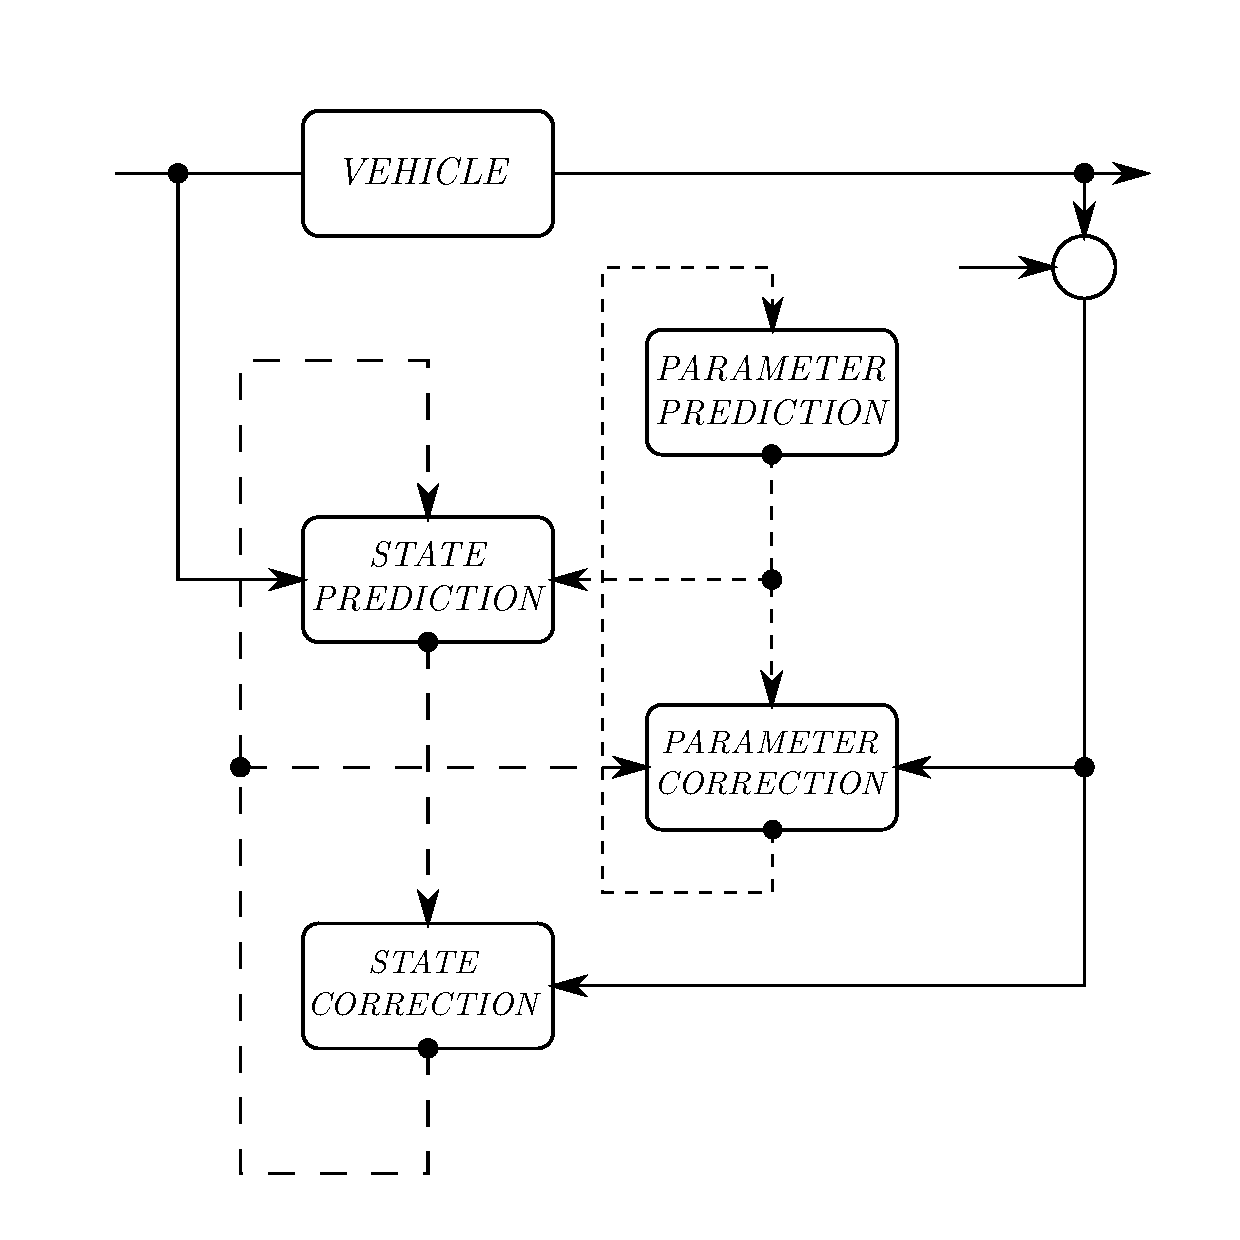
\includegraphics[scale = 0.5]{Images/flow.pdf}};
	\node at (30pt,270pt) {$\gamma$};
	\node at (270pt,270pt) {$\nu,\eta$};
	\node at (240pt,245pt) {$\sigma$};
	\node at (170pt,245pt) {$\bar{\mu}_\theta$};
	\node at (85pt,222pt) {$\bar{\mu}_s$};
	\node at (200pt,160pt) {$\hat{\mu}_\theta$};
	\node at (115pt,125pt) {$\hat{\mu}_s$};
	\node at (270pt,222pt) {$\nu_{meas},\eta_{meas}$};
	\end{tikzpicture}
	\caption{Online dual state and parameter estimation}
	\label{fig:Estimation_frame}
\end{figure}

Unscented Kalman filter is extension of Kalman filter for non-linear estimation. In UKF, the unscented transform is utilized. This involves deterministic extraction of sigma points from the Gaussian distribution and using these sigma points as an input to the nonlinear function \cite{wan}. The resultant Gaussian is also approximated from these transformed sigma points, thus the entire Kalman filter formulation remains the same. 

For the state and parameter, different sets of sigma points were selected based on - 

\begin{gather}
\chi^{[0]} = \mu \\
\chi^{[i]} = \mu + (\sqrt{(n+\lambda)\Sigma})_i \hspace{3pt} for \hspace{2pt}i=1,...,n \\
\chi^{[i]} = \mu - (\sqrt{(n+\lambda)\Sigma})_{i-n} \hspace{3pt} for \hspace{2pt}i=n+1,...,2n
\end{gather}

where $\mu$ denotes either the the combined state vector $[\nu_{meas},\eta_{meas}]^T$ or $\theta$, $n$ is the dimension the either state and parameter vector. The term $\lambda$ is given by $\lambda = \alpha^2(n+\kappa)-n$, with $\alpha$ and $\kappa$ are scaling parameter and reflect where the sigma points are selected in the Gaussian distribution. Adding to this, each sigma points have an associated weight as well which helps to regenerate the Gaussian distribution from sigma points.
  
\begin{gather}
w_m^{[0]} = \frac{\lambda}{(\lambda+n)} \\
w_c^{[0]} = \frac{\lambda}{(\lambda+n)} + (1-\alpha^2+\beta) \\
w_m^{[i]} = w_c^{[i]} = \frac{1}{2(n+\lambda)} \hspace{3pt}for \hspace{2pt}i = 1,..,2n 
\end{gather}

the sigma points are passed to the RK4 integration function of the hovercraft model $f_\nu, f_\eta$ for the update step. The complete algorithm for Dual UKF is based \cite{Thrun}.

\section{Results \& Discussion}
\subsection{Simulation of Identification framework}
Extensive simulation of hovercraft dynamics and identification framework was performed to ensure the correctness of the implementation. An artificial identification data was generated in simulation with known parameters defined as $\theta_{true}$. The identification input was chosen to be \texttt{PBRS} signal of varying frequency in the range 10-50 Hz. A synthetic Gaussian random noise was also added to the simulated position and velocity trajectory to account for real world noise. The estimated parameters from both the framework using the artificial data is presented in Table.\ref{simResults}.

\begin{center}
\begin{longtable}[c]{|c|c|c|c|c|}
\hline \rowcolor{gray!30}
 & $I_z$ & $X_u$ & $Y_v$ & $N_r$ \\ \hline
\endfirsthead
\endhead
True Value & 0.0001 & 0.05 & 0.048 & 0.0001  \\ \hline
Initial Guess & 0.01 & 0.2 & 0.25 & 0.005 \\ \hline
Offline Estim. & 0.0001 & 0.0497 & 0.0470 & 0.0001 \\ \hline
Online Estim. & 0.0003 & 0.152 & 0.0529 & 0.0002 \\ \hline
\caption{Simulation results of the identification framework}
\label{simResults}
\end{longtable}
\end{center}

The online identification implementation also provides the evolution of the parameter estimation, this is presented in the following figures for the simulation experiment. 
\begin{figure}[H]
\begin{minipage}{.5\textwidth}
  \centering
    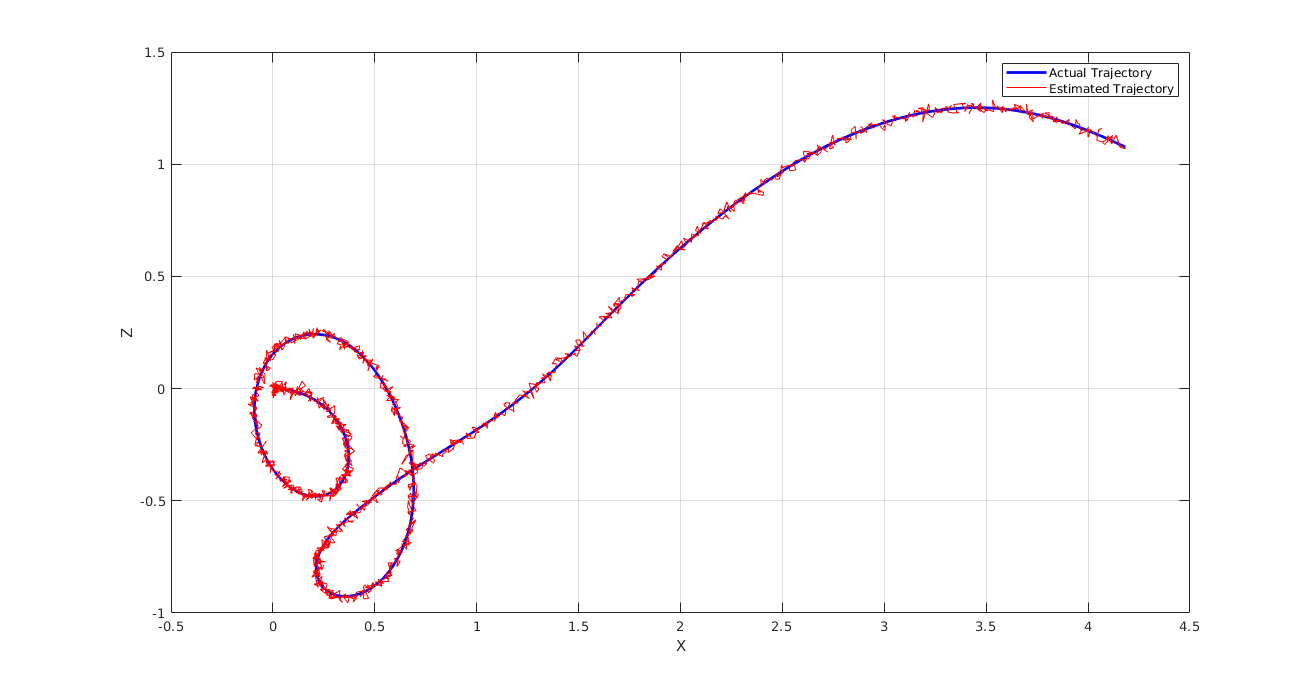
\includegraphics[width=0.9\columnwidth]{Images/state_estimate.png}\\
    \caption{Simulated trajectory and measure trajectory using PBRS input}
    \label{fig:ukf_traj_sim}
    \end{minipage}%
\begin{minipage}{.5\textwidth}
  \centering
    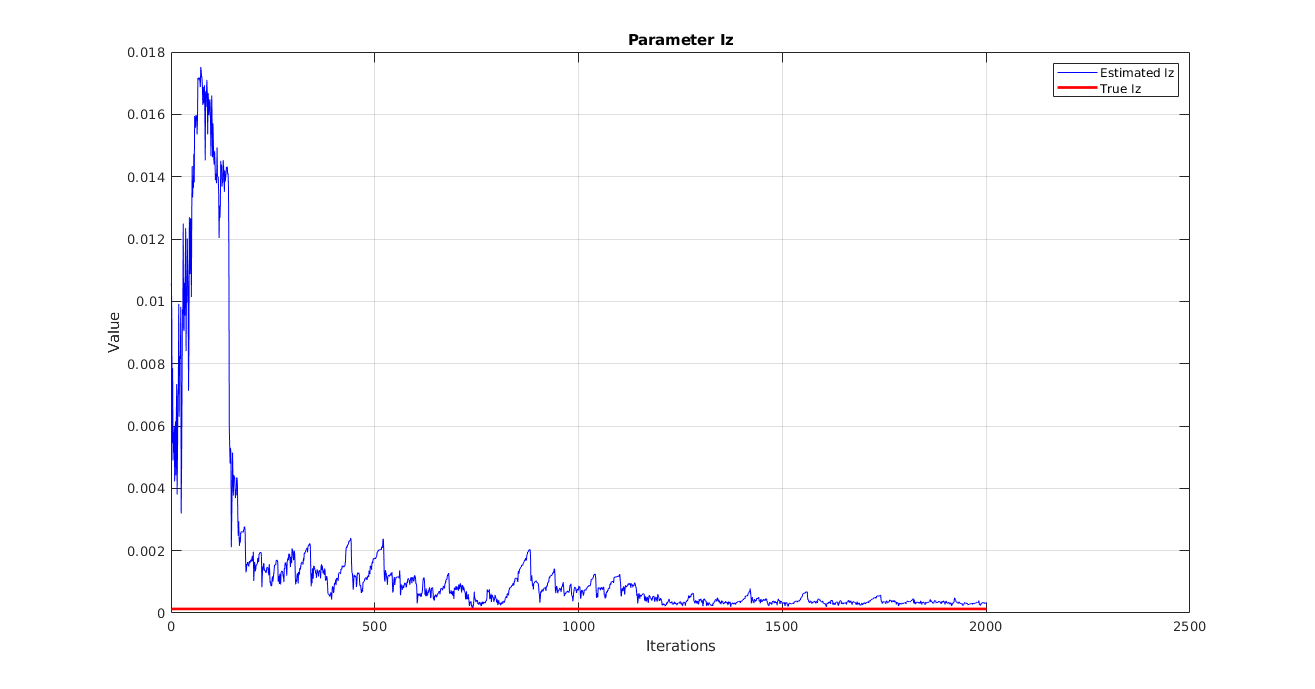
\includegraphics[width=0.9\columnwidth]{Images/Iz_param_plot.png}\\
    \caption{Evolution of $I_z$ parameter with iteration}
    \label{fig:ukf_Iz_sim}
    \end{minipage}%
\end{figure}

\begin{figure}[H]
\begin{minipage}{.5\textwidth}
  \centering
    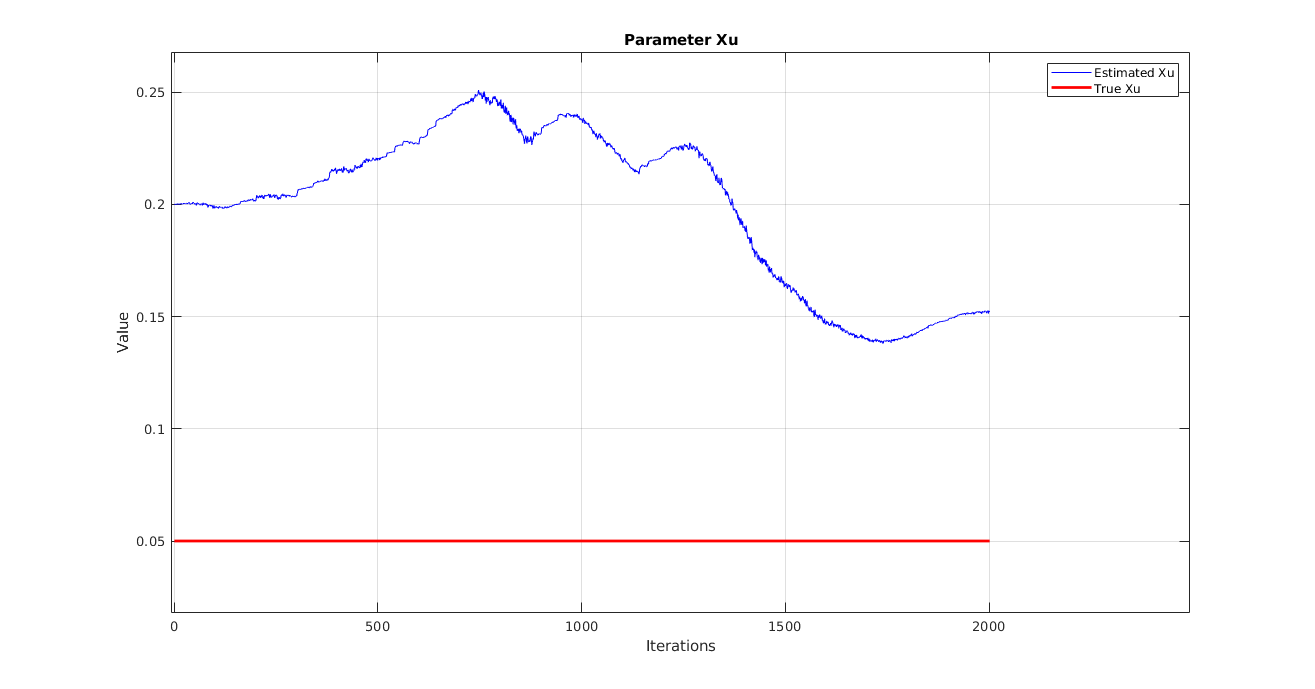
\includegraphics[width=0.9\columnwidth]{Images/Xu_param_plot.png}\\
    \caption{Evolution of $X_u$ parameter with iteration}
    \label{fig:ukf_xu}
    \end{minipage}%
\begin{minipage}{.5\textwidth}
  \centering
    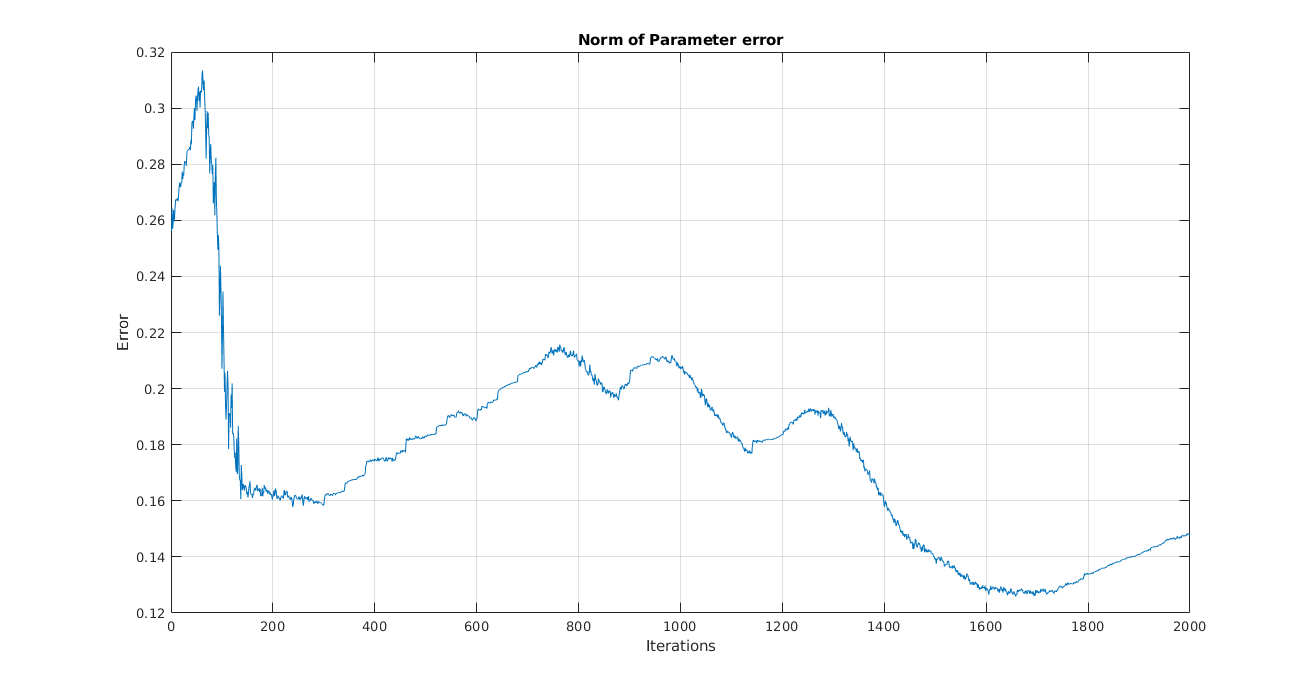
\includegraphics[width=0.9\columnwidth]{Images/Norm_param.png}\\
    \caption{Norm of the $\theta_{esti}$ and $\theta_{true}$}
    \label{fig:norm}
    \end{minipage}%
\end{figure}
However, as seen from the Table.\ref{simResults} and Figs.[\ref{fig:ukf_traj_sim}-\ref{fig:norm}], the convergence of the estimated parameter to true parameters $\theta_{true}$ using online method is sub-par compared to the offline method. This can be justified by the fact that, offline method explicitly utilises the complete data set to optimize the parameter estimation, however in online method, the effect of previous data is encoded in the co-variance matrix of the Gaussian distribution of the parameters, and measurement from each time instant is used to correct both the state and parameter. Additionally, dual UKF formulation provides a substantial list of tuning variables, which makes it a time consuming process to obtain reasonable results. 


\subsection{Experiments}
Actual identification experiment on the developed prototype of the hovercraft model was performed to validate the developed framework.

\subsubsection{Input to Thrust mapping}
In order to determine the amount of thrust the propellers provided at different rpm or more specifically input PWM values, an experimental mapping process was used. Fig.\ref{fig:experim_motor} shows the testbench, where PWM values were sequentially incremented and the thrust generated was measured using the weighing scale. \textsc{matlab's} curve fitting toolbox was used to generate a suitable mapping, as shown in Fig.\ref{fig:data_motor}. It was found that the mapping was slightly nonlinear and thus a  quadratic function was used to approximate the mapping instead of a linear function. 

\begin{figure}[H]
\begin{minipage}{.4\textwidth}
  \centering
    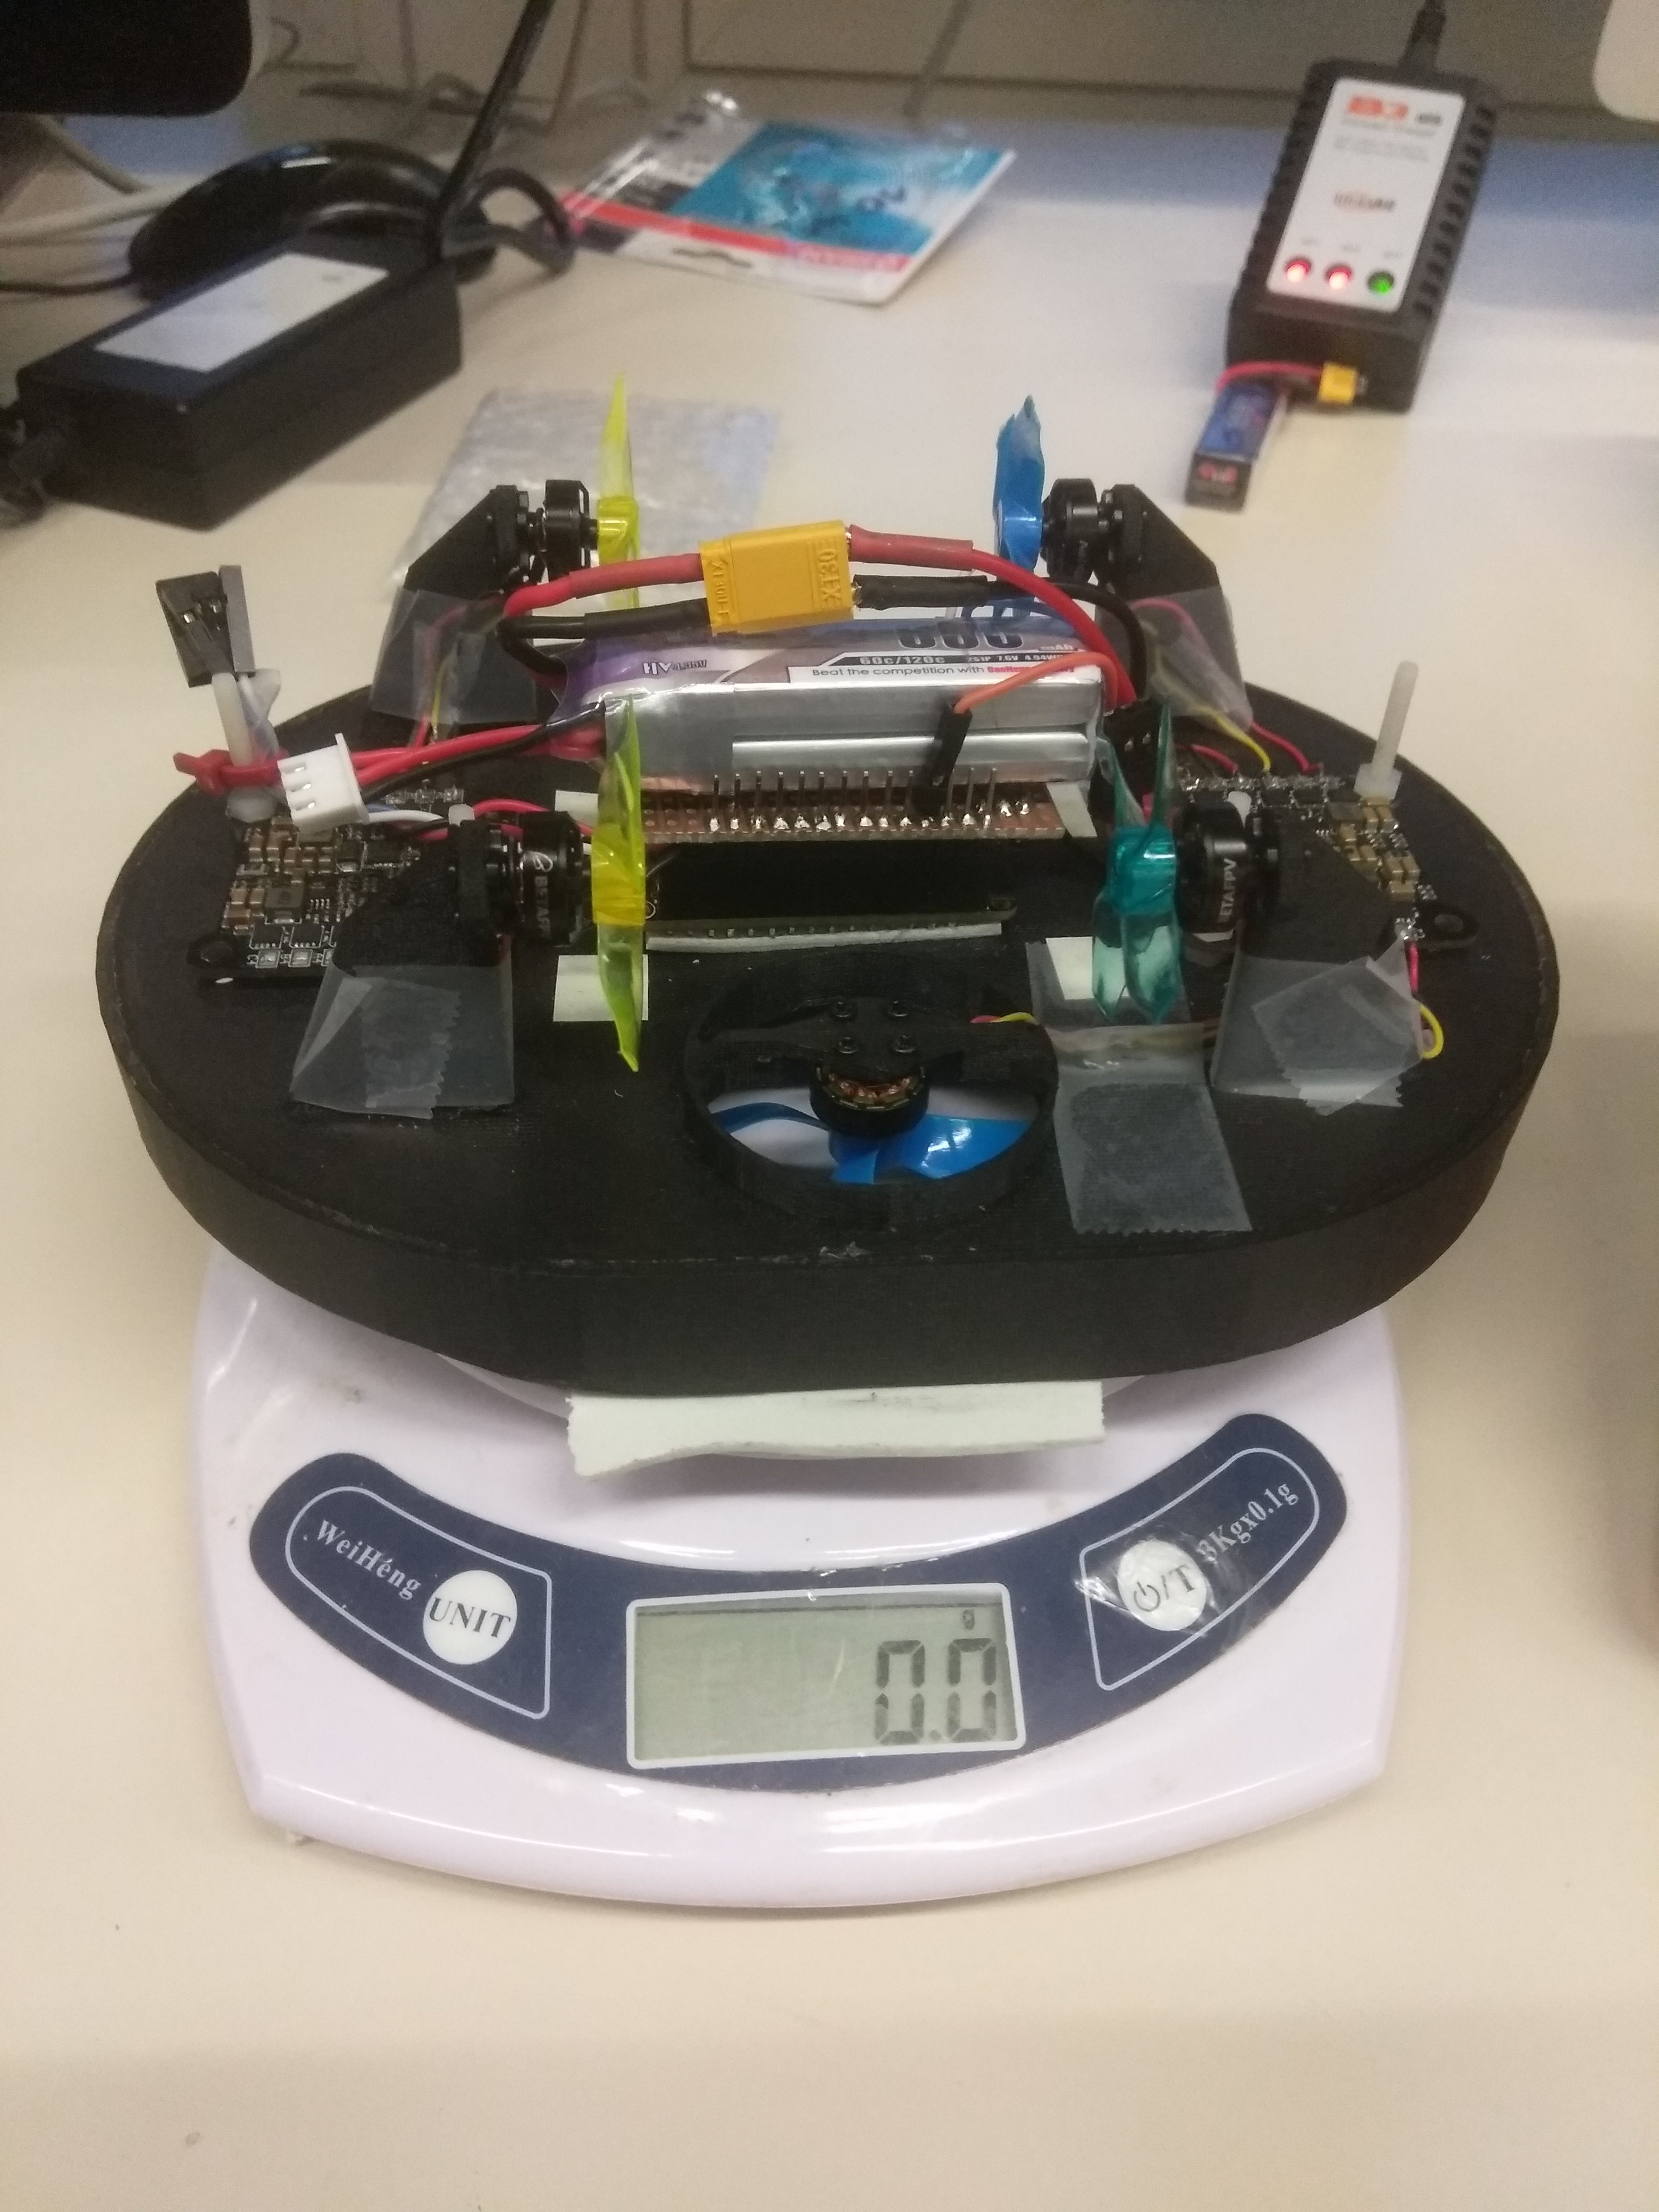
\includegraphics[width=0.6\columnwidth]{Images/motor_torque.jpg}\\
    \caption{Testbench for input to thrust mapping}
    \label{fig:experim_motor}
    \end{minipage}%
\begin{minipage}{.6\textwidth}
  \centering
    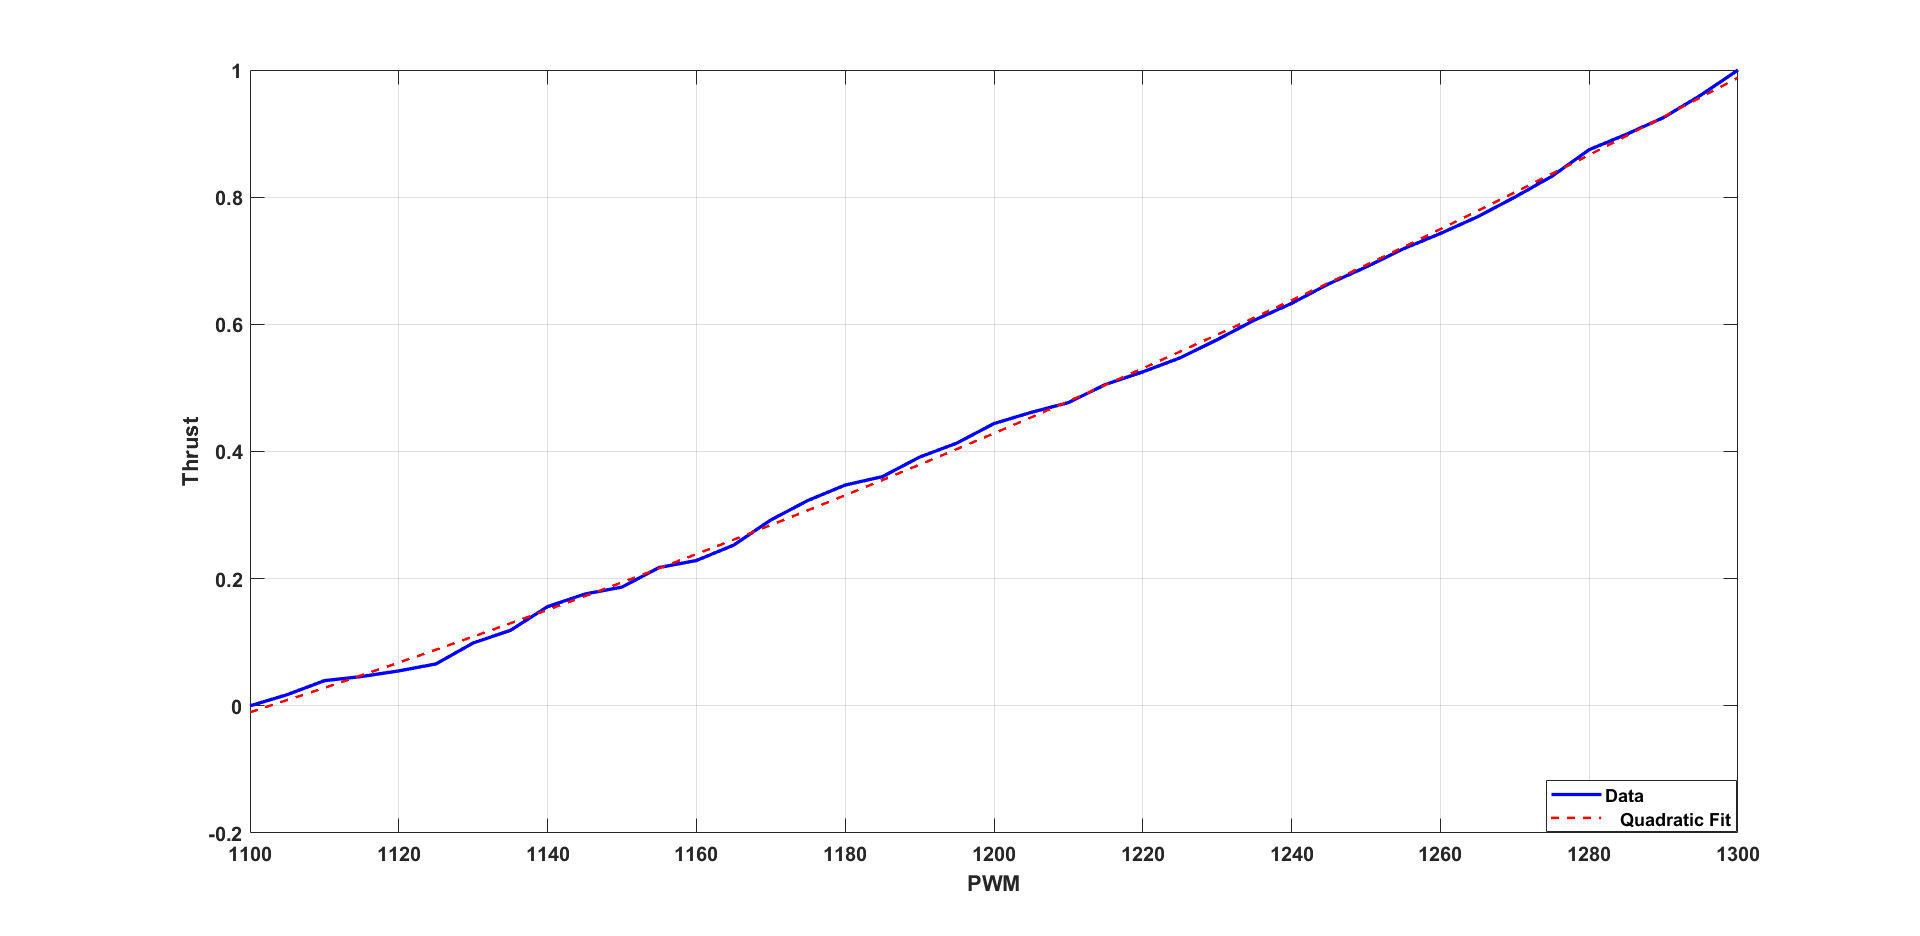
\includegraphics[width=1\columnwidth]{Images/motor_torque.png}\\
    \caption{Data Fitting}
    \label{fig:data_motor}
    \end{minipage}%
\end{figure}


\subsubsection{Parameter Identification}
Real experiments were performed to test the identification framework discussed in the previous section. In order to get the state measurements of the hovercraft, \textsc{Optitrack} motion tracking was used which provided the state ($\eta_{meas}, \nu_{meas}$) of the hovercraft. ROS served as the backbone and communication bridge between different elements of the setup. \texttt{mocap\_optitrack\_node} was used to obtain tracking data from the streaming service of Optitrack Motive software into the ROS master PC running \texit{identification\_node}. The \texit{identification\_node} also sent PWM commands to the \textit{hovercraft\_node} and also logging the status message received from \textit{hovercraft\_node}. The entire experimental setup can be visualised in the Fig. \ref{fig:schematic_opti} and \ref{fig:exper_setup_opti}.

\begin{figure}[H]
\begin{minipage}{.5\textwidth}
  \centering
    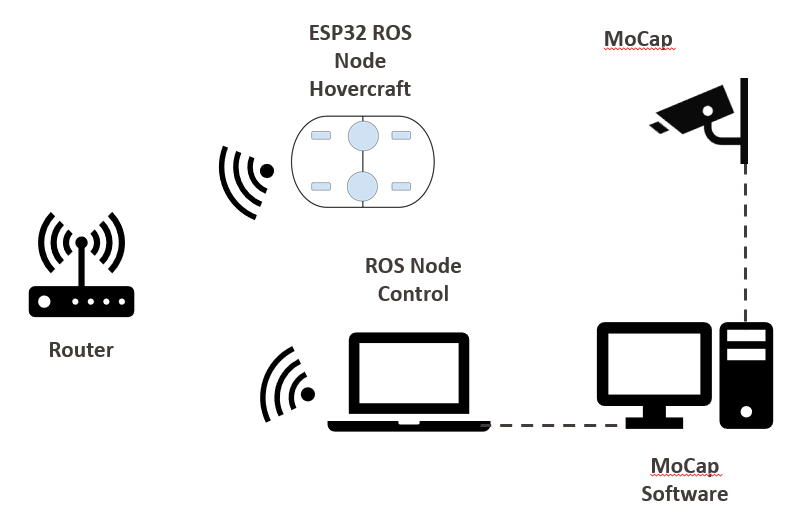
\includegraphics[width=0.9\columnwidth]{Images/experimental_setup.PNG}\\
    \caption{Schematic of the experimental setup}
    \label{fig:schematic_opti}
    \end{minipage}%
\begin{minipage}{.5\textwidth}
  \centering
    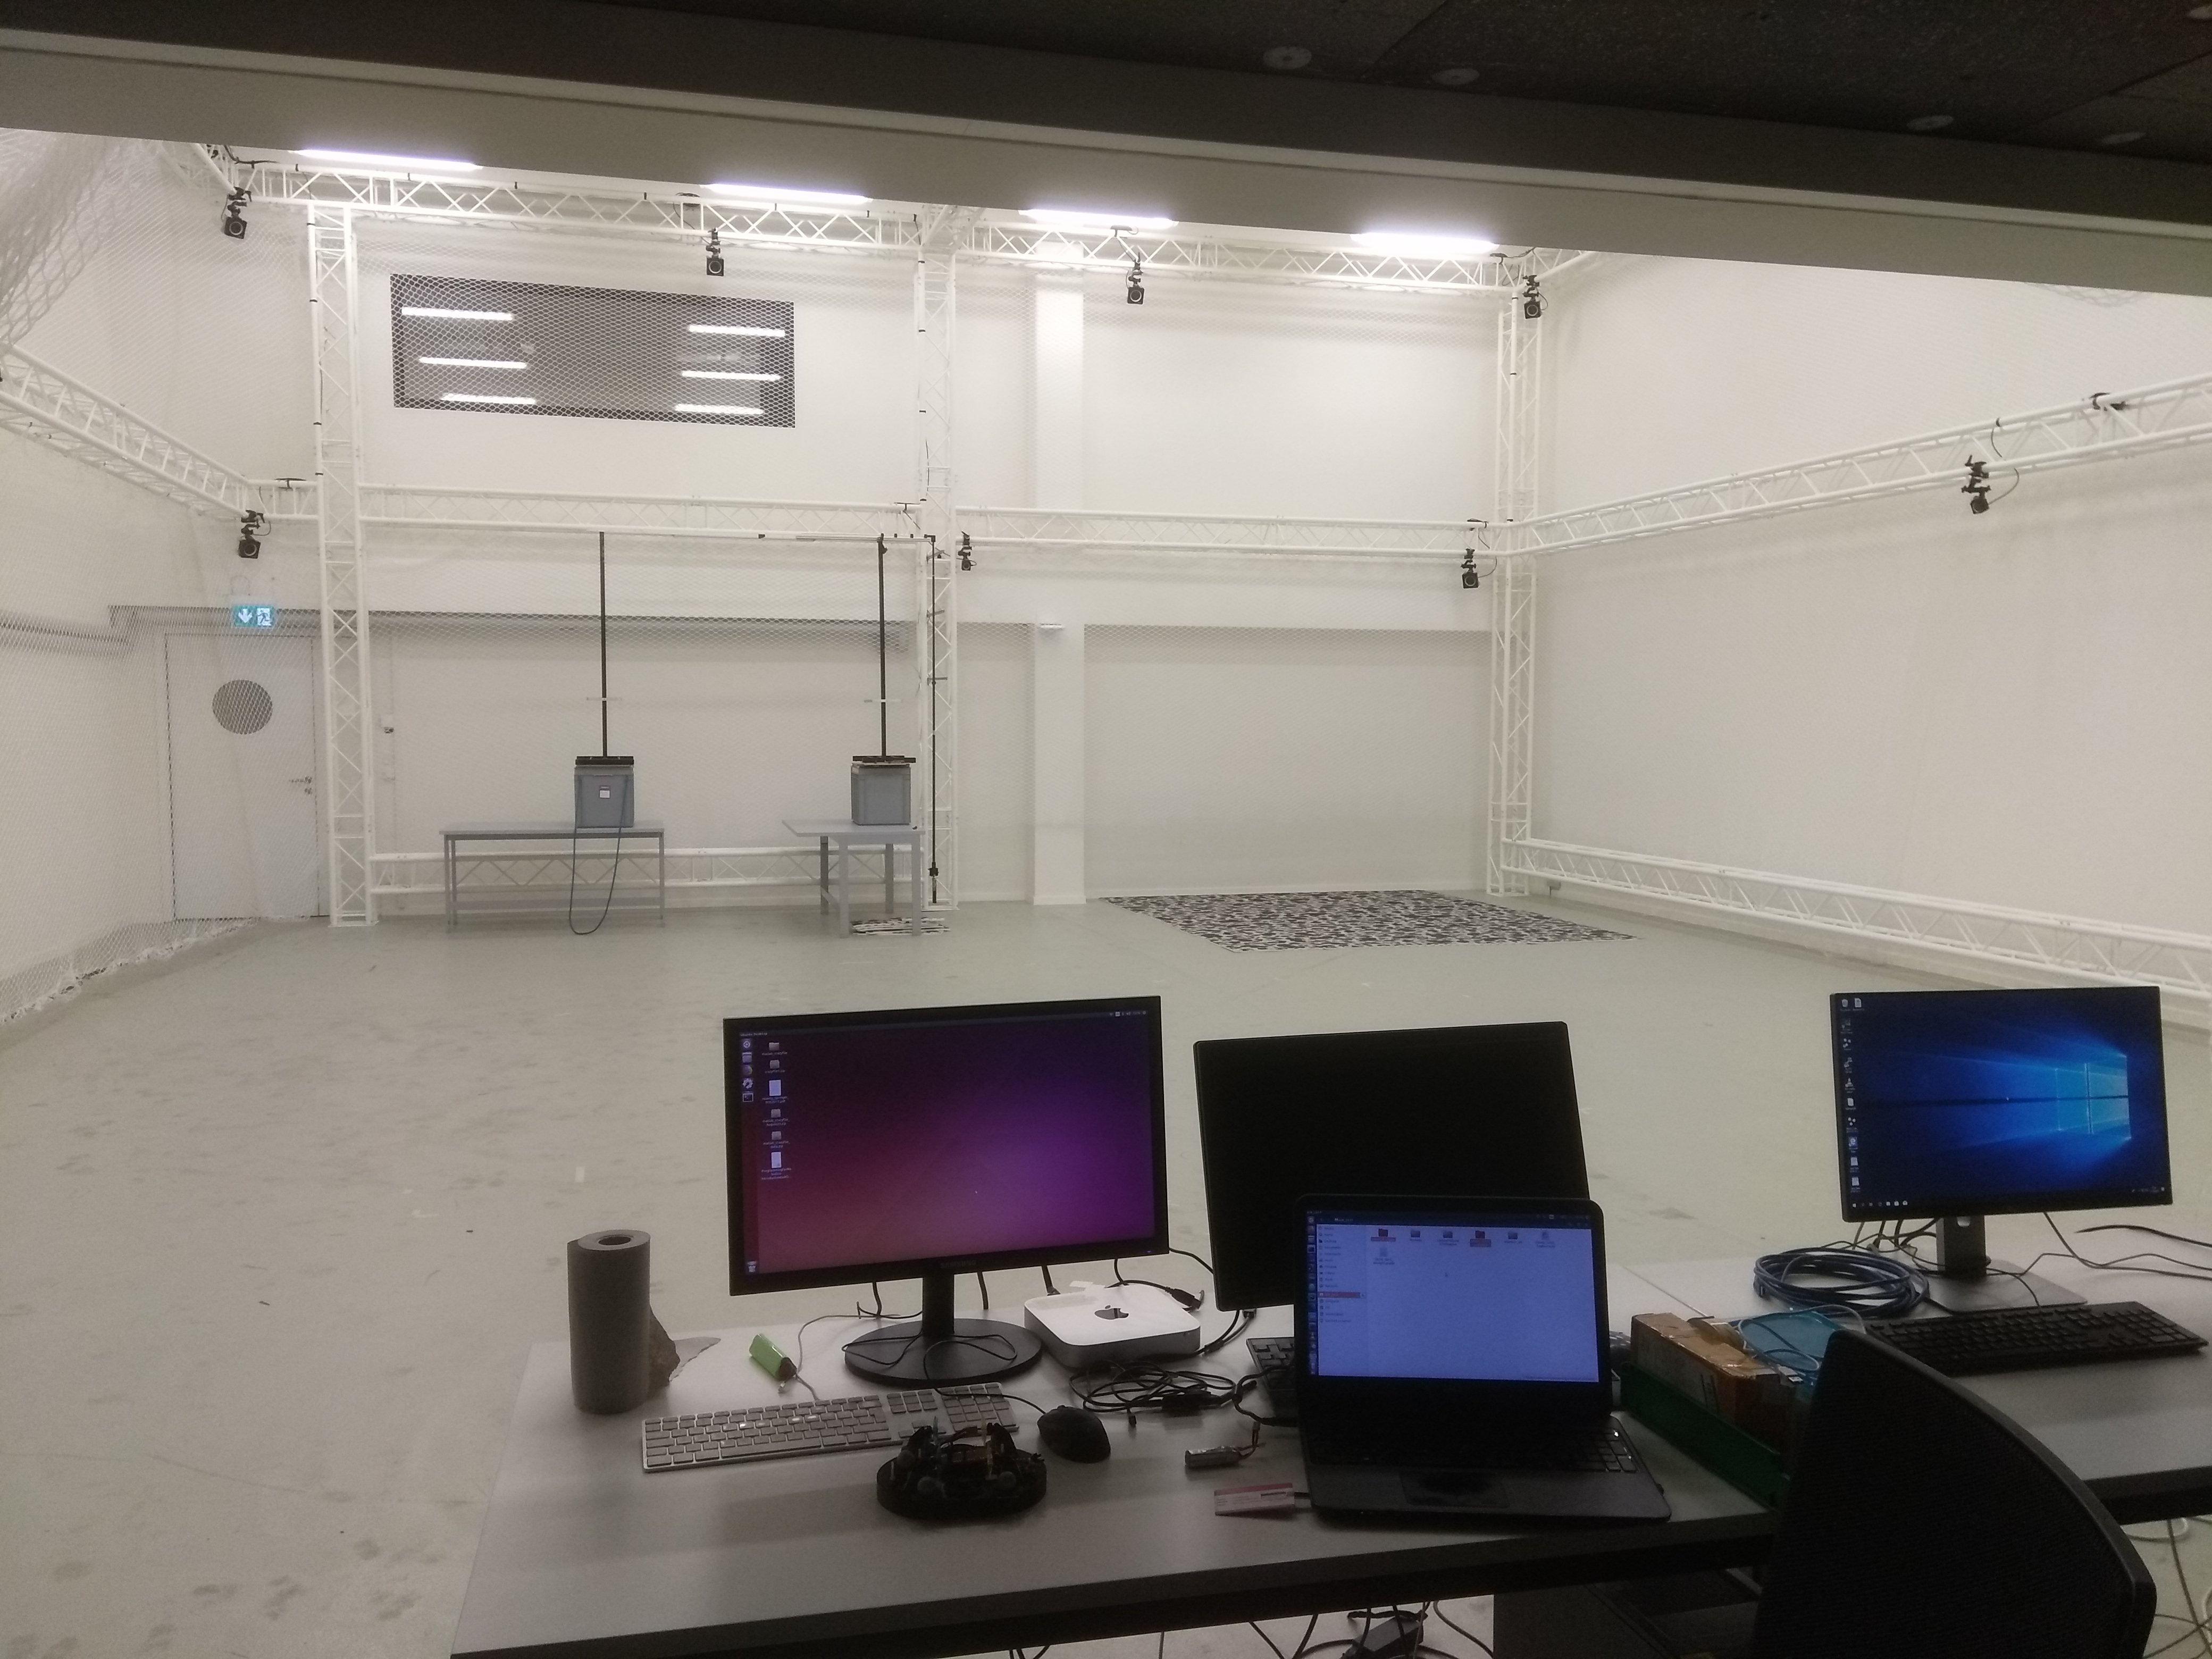
\includegraphics[width=0.9\columnwidth]{Images/experimental_setup.jpg}\\
    \caption{Optitrack motion tracking room and actual setup}
    \label{fig:exper_setup_opti}
    \end{minipage}%
\end{figure}
Different frequency of PBRS signal in the range 20-50 Hz was used to generate input data, and each set of repeated 3-4 times to ensure repeat ability. However, when the collected data was used in the identification framework to identify the parameters, it did not provide satisfactory results. In the online parameter estimation, the minimum of the optimization function seems to be stuck to a local minima, giving incredibly high values of the parameters. The simulated trajectory using the estimated parameters was far from the actual trajectory. Similarly, using the online parameter framework, the estimated parameters was abrupt and inconsistent. Even after repeated tuning of the UKF parameters such as initial covariance of the parameters, measurement noise lead to unsatisfactory results as shown in Fig.\ref{fig:ukfidentmodel}.

\begin{figure}[H]
    \centering
    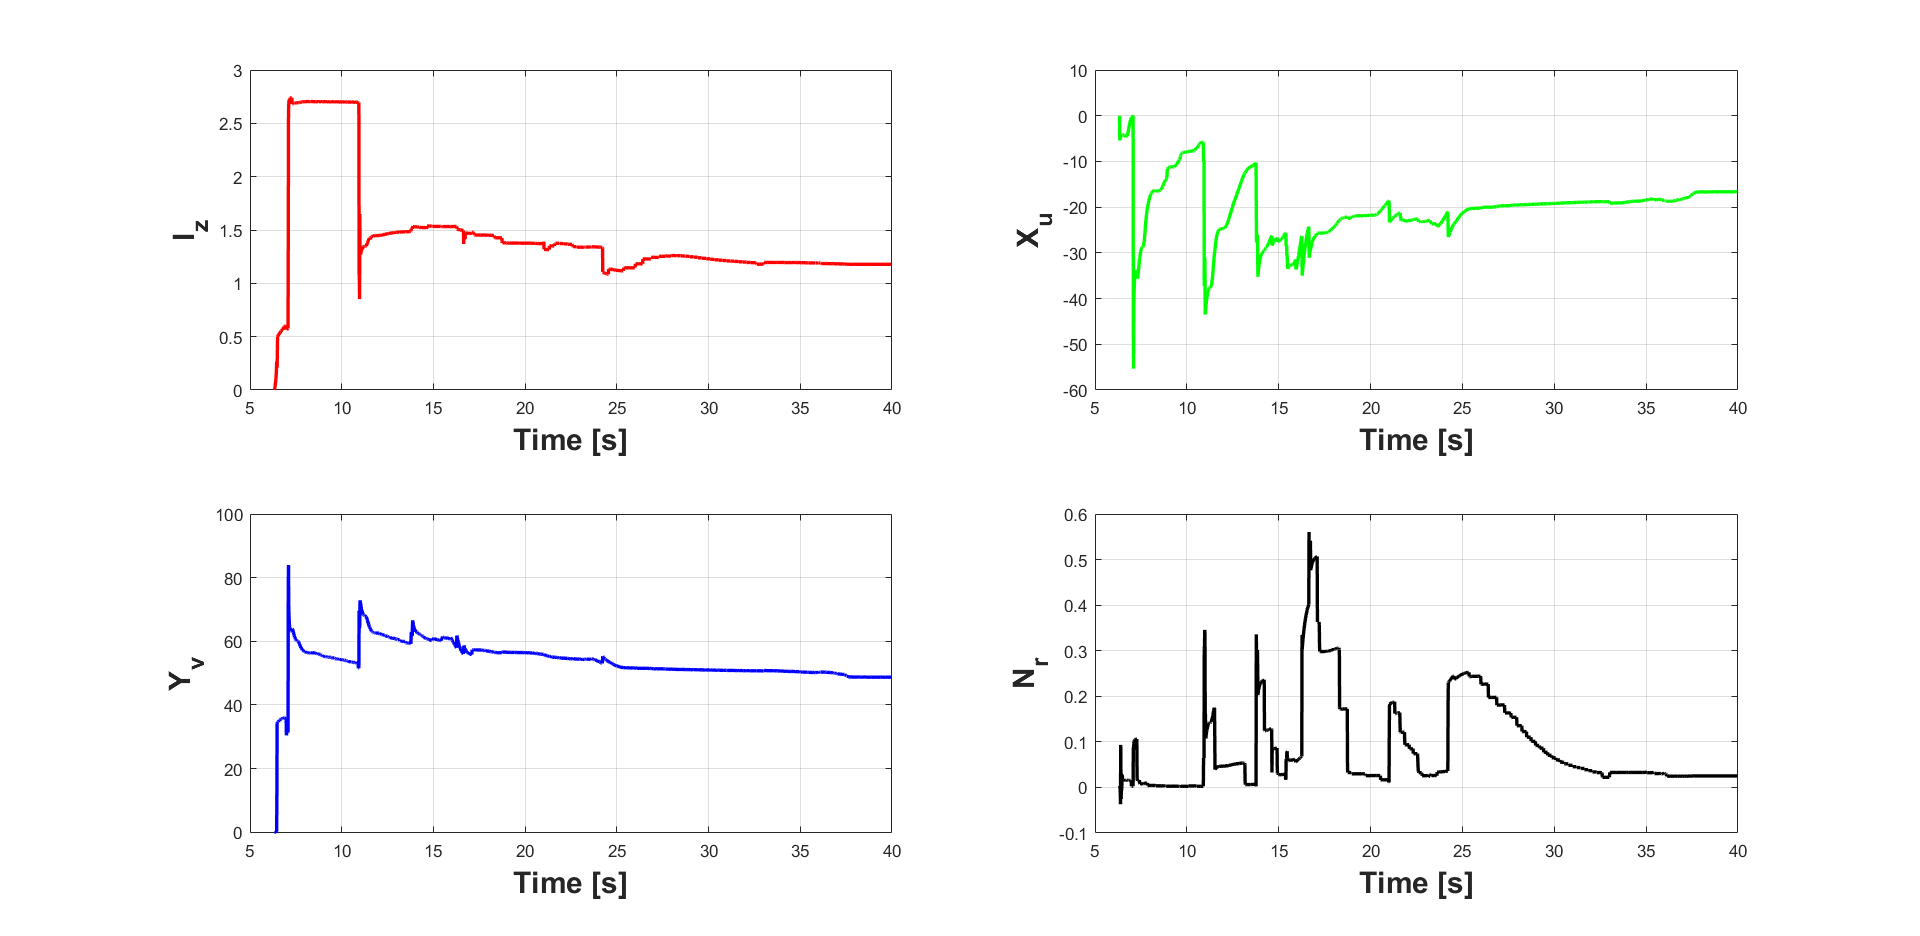
\includegraphics[width=1\columnwidth]{Images/param_ident_ukf.png}\\
    \caption{System model of the hovercraft}
    \label{fig:ukfidentmodel}
\end{figure}

There may be multiple reasonable reasons for it. After careful analysis, two prominent possible reasons are discussed - 

\subsection*{Unmodelled Dynamics}
The hovercraft behaved quite differently, when same inputs were provided in different runs. This is shown in Fig.\ref{fig:uncertain} where, the $\eta_{meas}$ clearly shows, drastic change in each run. This may be due to uneven and rough floor in the tracking room. Additionally, one of the shortcoming of the developed hardware was the inability to monitor battery level, thus with time, the amount of thrust provided by the lift propellers gradually decreased, thus making the damping parameters time varying. Therefore, it is quite difficult to estimate parameters using either offline or online identification framework formulated above as the mathematical model is not capable of handling such degree of uncertainty. 

\begin{figure}[H]
    \centering
    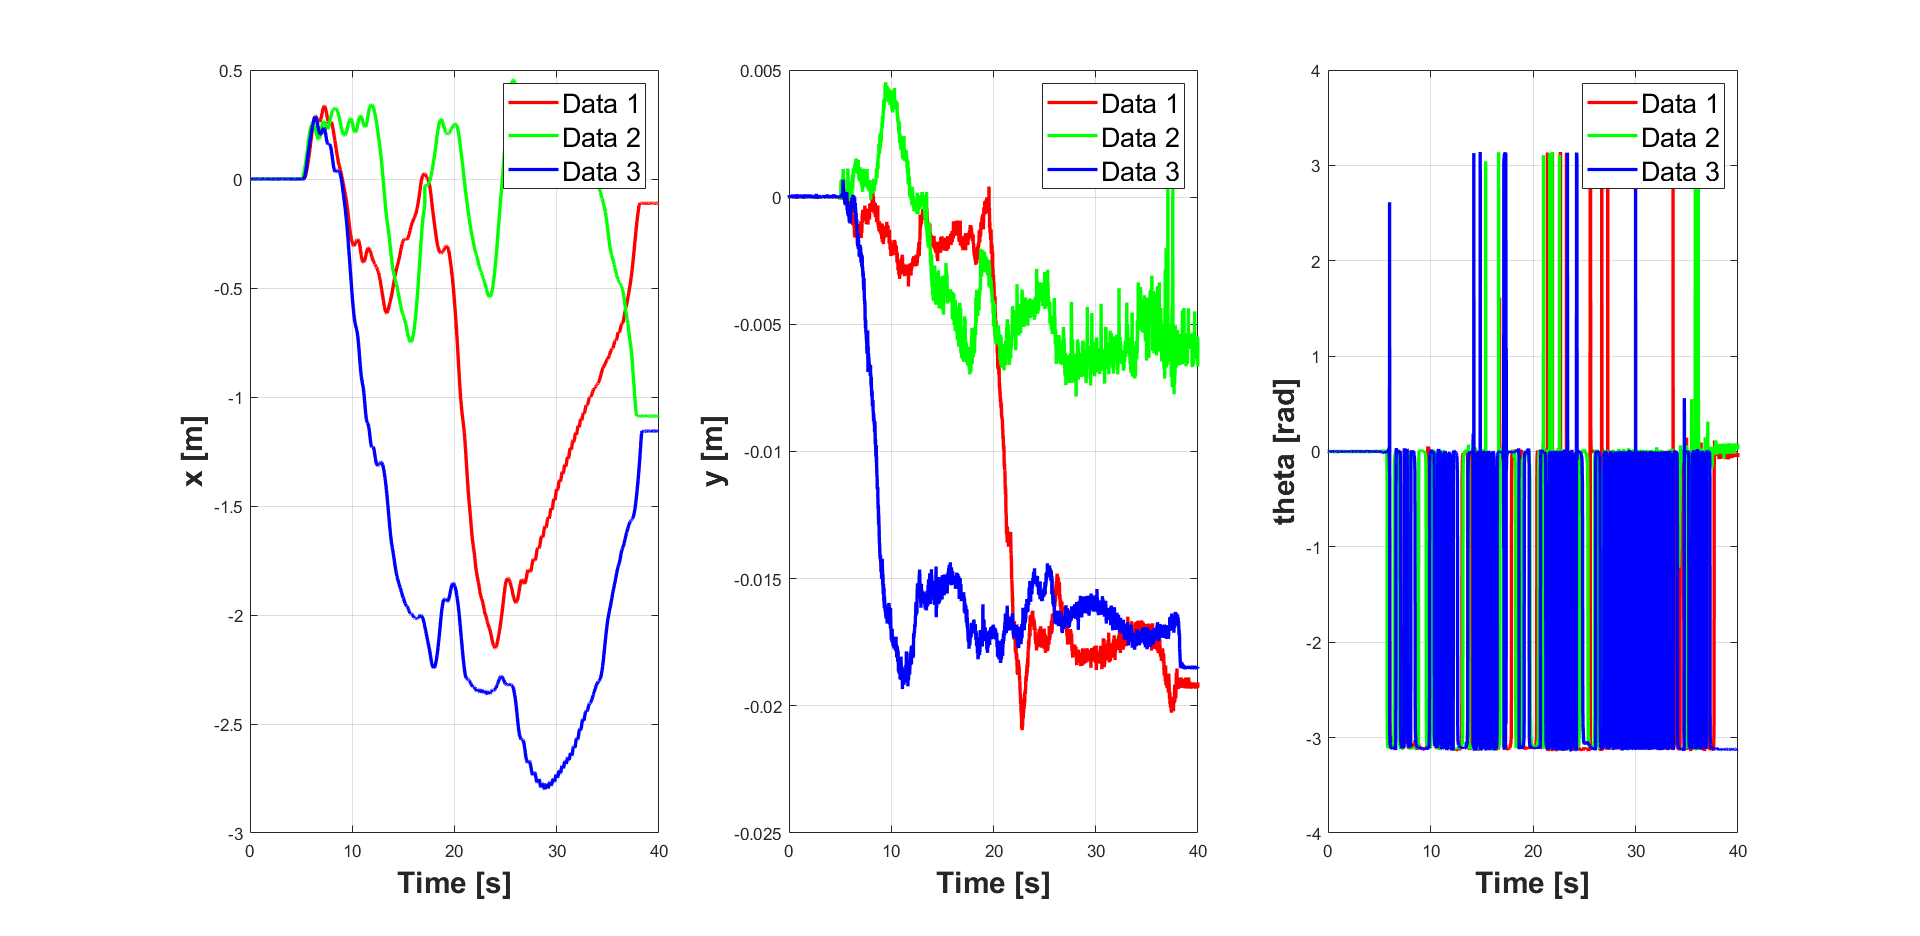
\includegraphics[width=1\columnwidth]{Images/dynamics_error.png}\\
    \caption{Uncertain dynamics of the hovercraft}
    \label{fig:uncertain}
\end{figure}

\subsection*{Network Lag}
Another possible reason for inefficient data collection could be attributed to the wireless network lag experienced by the experimental setup. As, the embedded firmware provided a time stamped hovercraft status under ROS environment, it provided a tool to analyse the network lag. The Fig.\ref{fig:networkLag} shows the slight time difference in the commanded PWM values sent and received, which is quite significant during the initial time. However, this lag was not accounted for when state measurements were recorded with the Optitrack tracking environment, thus creating discrepancy in the data collected during the experiment. 

\begin{figure}[H]
	\centering
	
	\begin{subfigure}{0.49\textwidth}
	\centering
	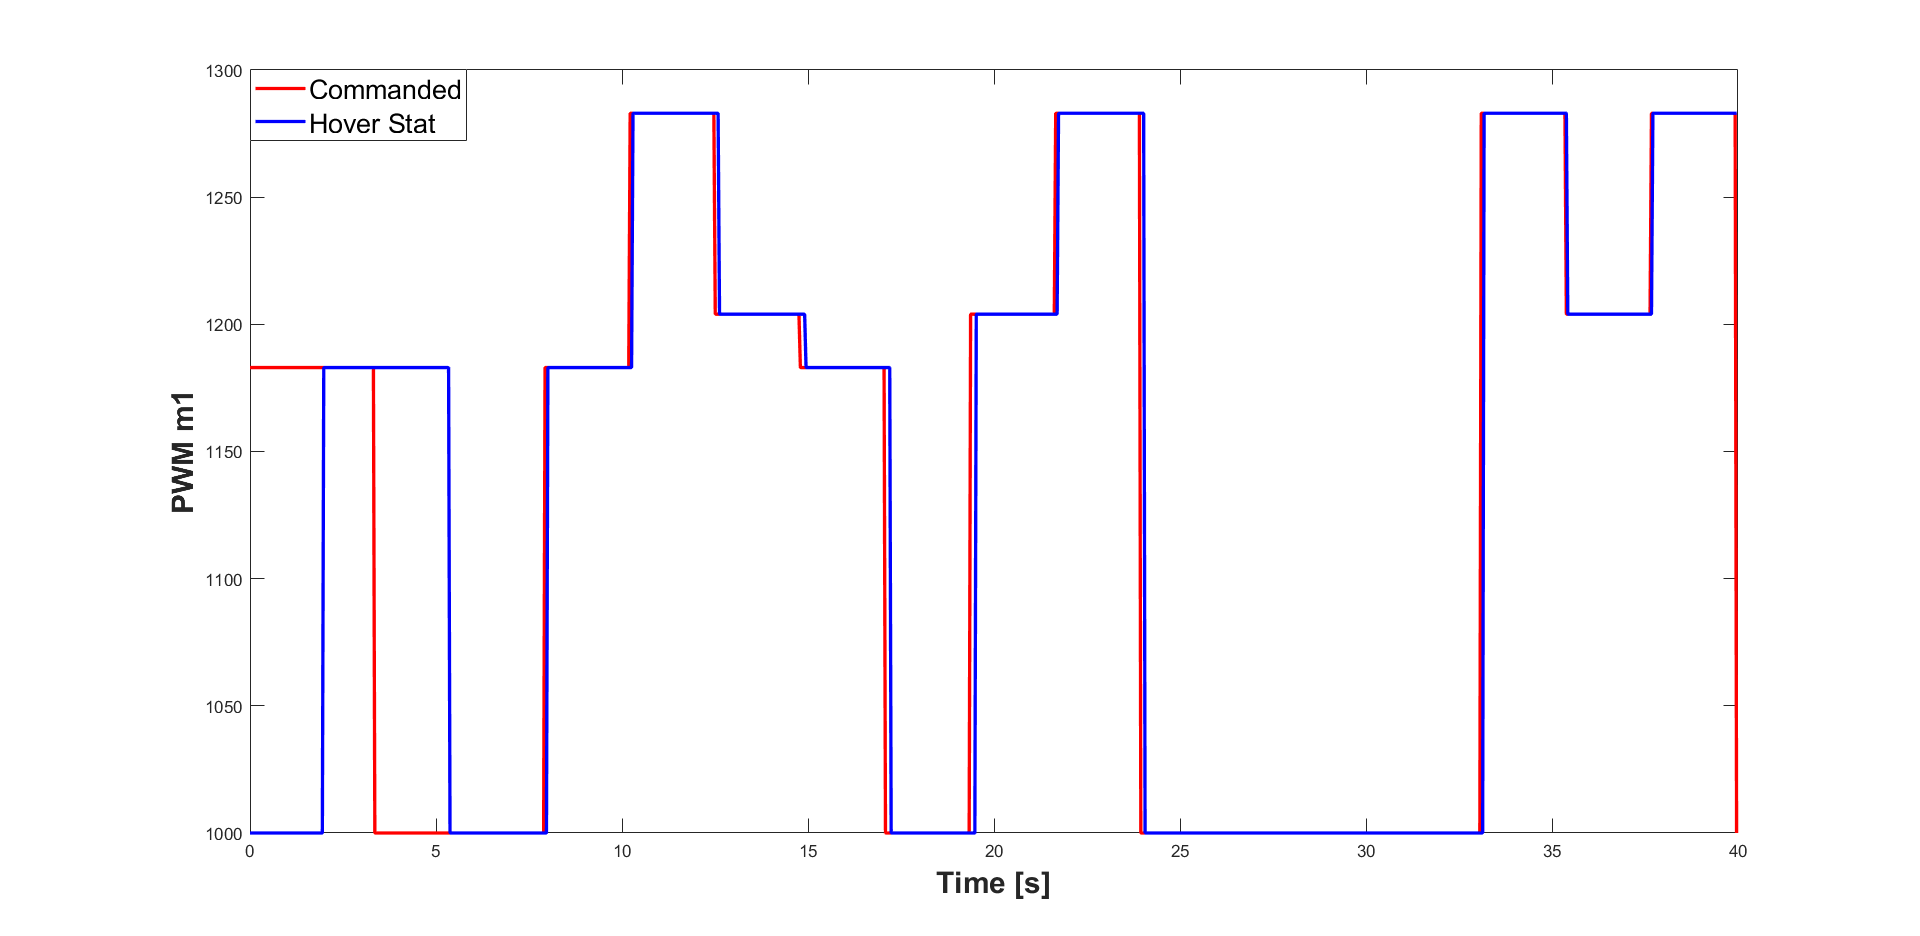
\includegraphics[width = \textwidth]{Images/lag_data_2_spec_2_m1.png}
	\end{subfigure}
	\begin{subfigure}{0.49\textwidth}
	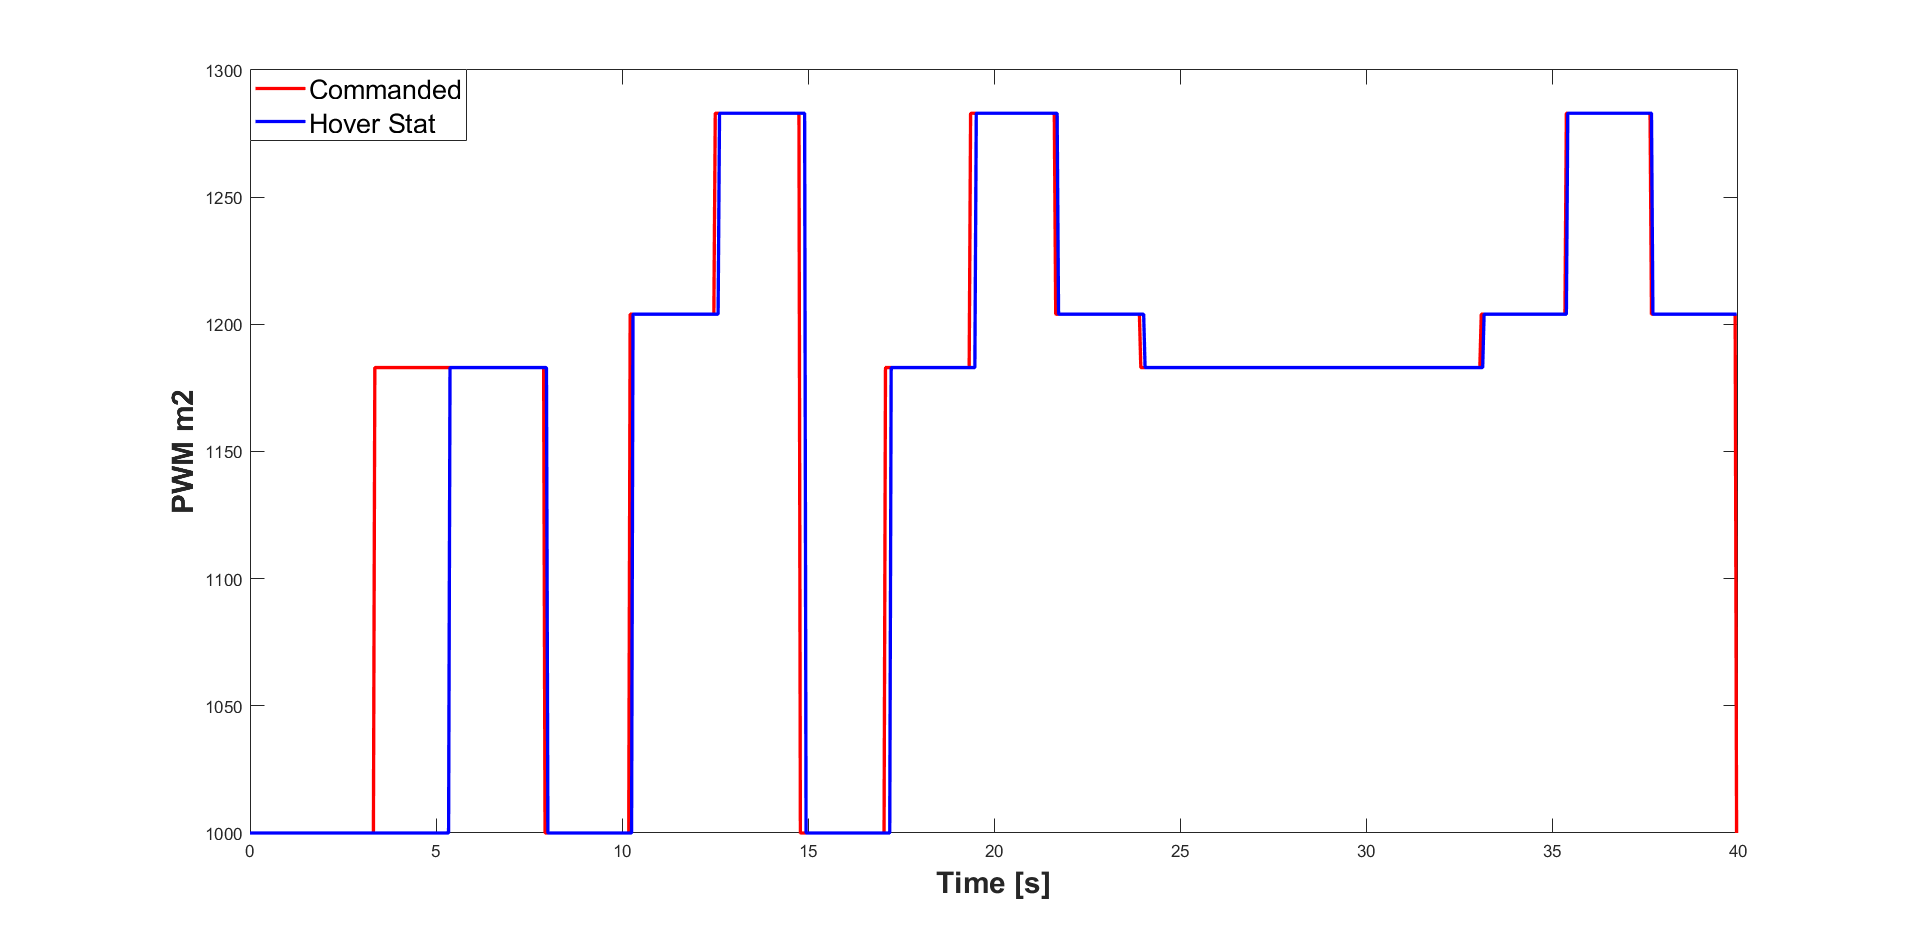
\includegraphics[width = \textwidth]{Images/lag_data_2_spec_2_m2.png}
	\end{subfigure}
    \begin{subfigure}{0.49\textwidth}
	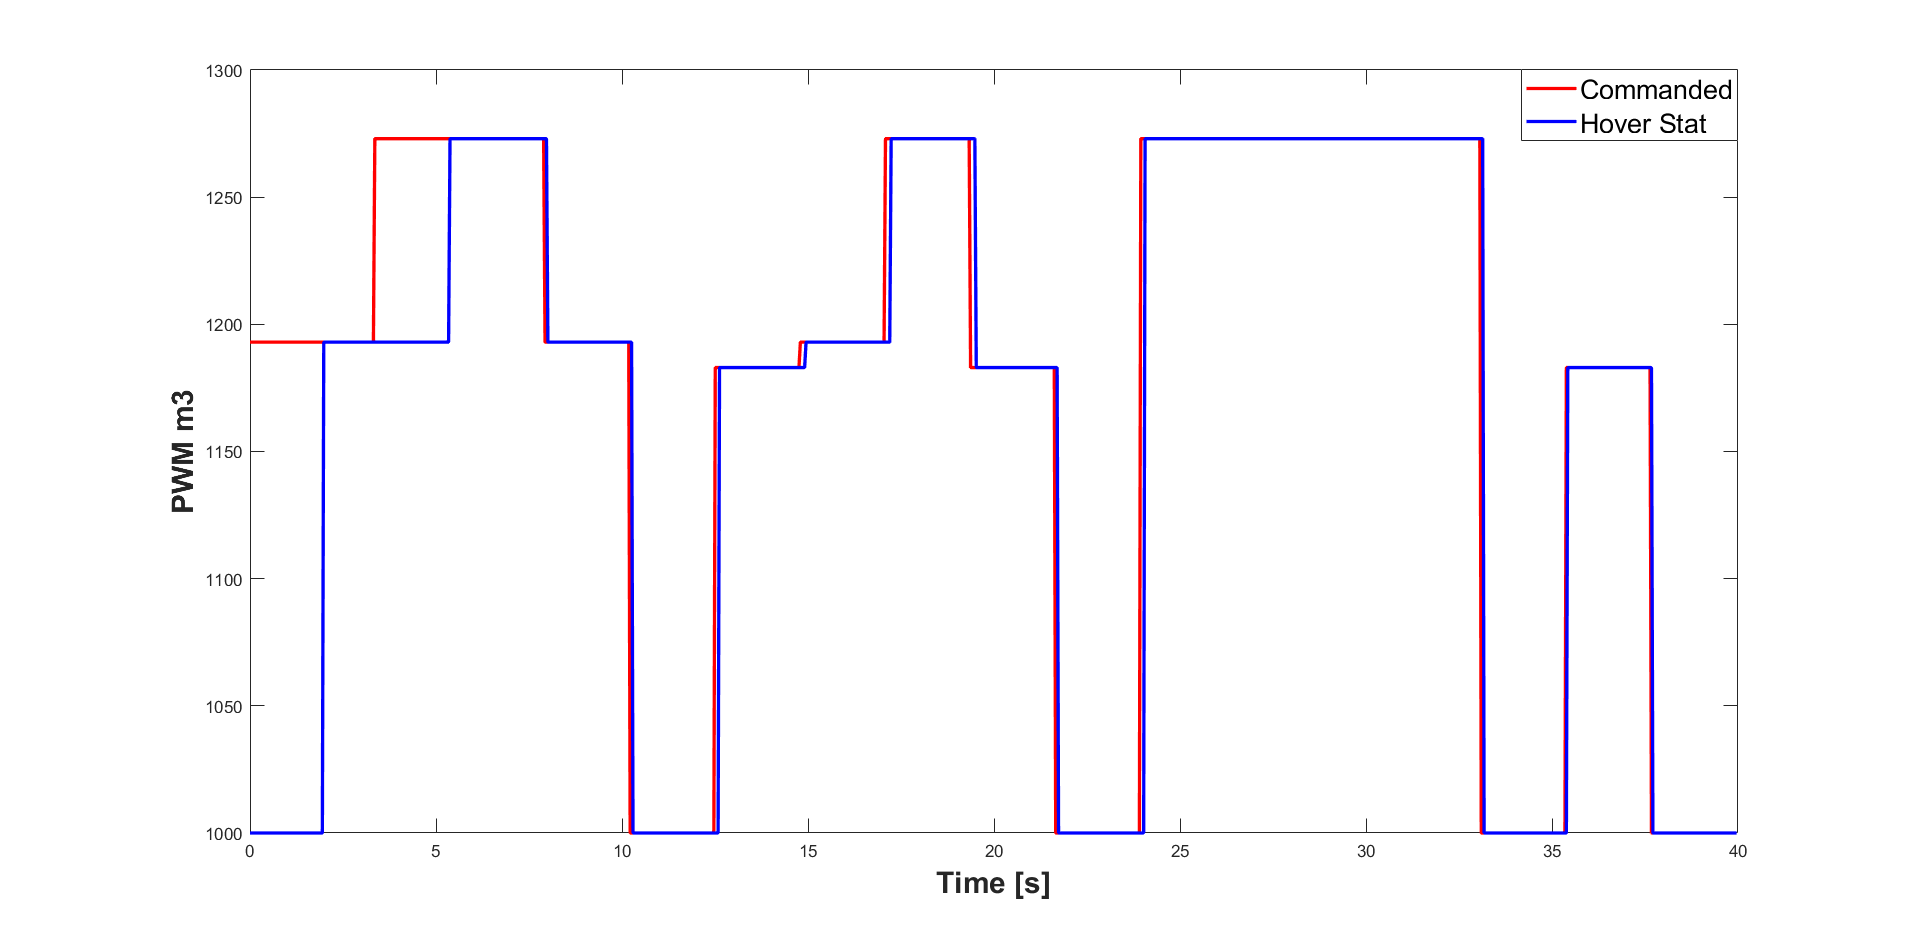
\includegraphics[width = \textwidth]{Images/lag_data_2_spec_2_m3.png}
	\end{subfigure}
	\begin{subfigure}{0.49\textwidth}
	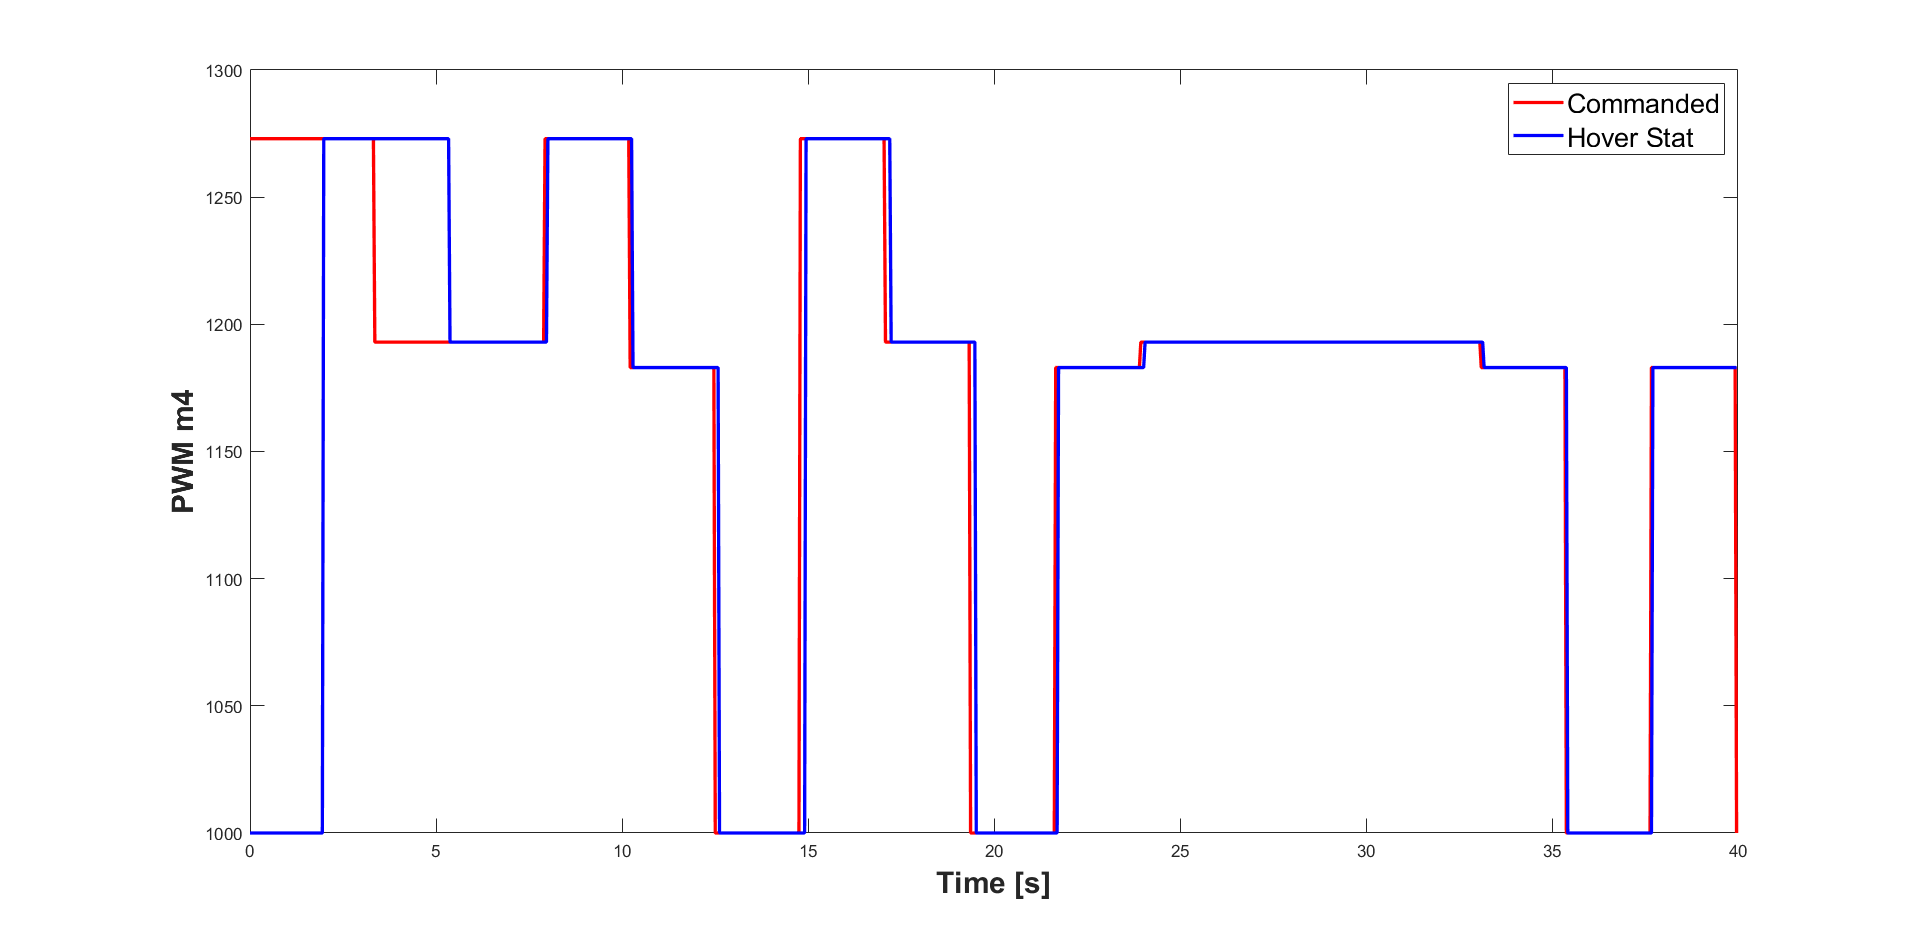
\includegraphics[width = \textwidth]{Images/lag_data_2_spec_2_m4.png}
	\end{subfigure}
    \caption{Lag in PWM commands send to each motor and the received status of the PWM command}
\label{fig:networkLag}
\end{figure}


\section{Conclusion}
In this project, the major contribution was development of a miniature prototype hovercraft which had the capability to provide forward, backward and lift thrust. The developed firmware and hardware prototype satisfied most of the design requirements. In terms of improvement, it would be essential to monitor the battery level and adjust the lift thrust so that the damping parameters are not time varying. Though, two prominent identification framework was implemented, it did not provide consistent and satisfactory results on actual experimental data, thus raising the question about the effectiveness of the framework in uncertain scenarios. Possible solutions could be model noise and uncertainty into the identification framework, making it robust and effective. Additionally, for control objective, data driven approach should be employed instead of traditional identification and control scheme.
\newline


\begin{thebibliography}{33}
	\expandafter\ifx\csname natexlab\endcsname\relax\def\natexlab#1{#1}\fi
	\expandafter\ifx\csname url\endcsname\relax
	\def\url#1{\texttt{#1}}\fi
	\expandafter\ifx\csname urlprefix\endcsname\relax\def\urlprefix{URL }\fi


	\bibitem{b1}
    T. I. Fossen, Guidance and control of ocean vehicles. John Wiley & Sons Inc, 1994.

	\bibitem{b2}
    Identification and control of a miniature hovercraft, Mauro Pfister, July 2019.

    \bibitem{b3}
    Eric A. Wan, Rudolph van der Merwe, Alex T. Nelson "Dual Estimation and the Unscented Transformation"
    
    \bibitem{Thrun}Thrun, S., Burgard, W.,, Fox, D. (2005). Probabilistic robotics. Cambridge, Mass.: MIT Press. ISBN: 0262201623 9780262201629 
		
\end{thebibliography}

\end{document}

